



%--------------------------------------


\newpage

%\section[Network Growth Models][Modèles de Croissance de Réseau]{Network Growth Models : Explicative power for various approaches}{Modèles de Croissance de Réseau}
\section{Network growth models}{Modèles de croissance de réseau}


\label{sec:networkgrowth}


%--------------------------------------


\bpar{
We propose first to study with more details processes of network growth for the mesoscopic sclae. The idea is to understand intrinsic properties of different network growth heuristics. This exercise is interesting in itself since there is to the best of our knowledge no systematic comparison of spatial networks morphogenesis models: \cite{xie2009modeling} propose for example a review from the point of view of network economics, it does not include on the one hand some disciplines (see chapter~\ref{ch:modelinginteractions}), and on the other hand does not compare performances of models on dedicated comparable implementations.
}{
Nous proposons dans un premier temps d'étudier en détails les processus de croissance de réseau pour l'échelle mesoscopique. L'idée est de comprendre les propriétés intrinsèques des différentes heuristiques de croissance de réseau. Cet exercice est intéressant en lui-meme puisqu'il n'existe pas à notre connaissance de comparaison systématique de modèles de morphogenèse des réseaux spatiaux : si~\cite{xie2009modeling} proposent par exemple une revue du point de vue de l'économie des réseaux, celle-ci ne prend pas en compte certaines disciplines d'une part (voir chapitre~\ref{ch:modelinginteractions}), et ne compare d'autre part pas les performances des modèles sur des implémentations dédiées comparables. 
}



%--------------------------------------

%%%%%%%%%%%%%%%%%%%%
\subsection{Benchmarking network growth heuristics}{Comparer les heuristiques de croissance de réseau}


\bpar{
Considering network growth in itself, several heuristics exist in order to generate a network under some constraints. As already developed especially in~\ref{sec:modelingsa}, from economic network growth approaches to local optimization heuristics, geographical mechanisms or biological network growth, each has its own advantages and particularities. We already tested in~\ref{sec:correlatedsyntheticdata} an heuristic based on interaction potential breakdown. In order to be able to compare different network growth heuristics ``everything else being equal'', it is necessary to explore them at fixed density, although the thematic meaning of results will not have any value, neither on long times nor for co-evolution.
}{
Pour la croissance du réseau en tant que telle, de nombreuses heuristiques existent pour générer un réseau sous certaines contraintes. Comme déjà développé précédemment notamment en~\ref{sec:modelingsa}, des modèles économiques de croissance de réseau aux heuristiques d'optimisation locale, aux mécanismes géographiques ou à la croissance de réseau biologique, chacun a ses avantages et particularités propres. Nous avons déjà testé en~\ref{sec:correlatedsyntheticdata} une heuristique basée sur la rupture de potentiel d'interaction. Pour pouvoir comparer ``toutes choses égales par ailleurs'' les différentes heuristiques de génération de réseau, il est nécessaire de les explorer à densité fixée, même si le sens thématique des résultats ne peut avoir de valeur ni sur le temps long, ni pour la co-évolution.
}


\bpar{
The importance of heuristics capturing a topological structure allowing a certain compromise between performance, congestion and cost, is shown by empirical analyses such as \cite{2012arXiv1202.1747W} for metropolitan networks, which shows that patterns of evolution for correlations between degrees witness an evolution of networks towards such a topology.
}{
L'importance d'heuristiques pouvant capturer une structure topologique permettant un certain compromis entre performance, congestion et coût, est montrée par des analyses empiriques comme \cite{2012arXiv1202.1747W} pour les réseaux de métro, qui montre que les motifs d'évolution des corrélations entre degrés témoignent d'une évolution des réseaux vers une telle topologie.
}


\bpar{
We precise in the following the core of the network growth model together with several heuristics from diverse origins, compared in similar conditions through their integration within the common basis.
}{
Nous précisons par la suite le coeur du modèle de croissance de réseau ainsi qu'un certain nombre d'heuristiques aux origines variées, comparées dans des conditions similaires par leur intégration à la base commune.
}



%%%%%%%%%%%%%%%%%%%%%%%
\subsubsection{Core of the network growth model}{Base du modèle de croissance de réseau}


\bpar{
A common process to the different heuristics constitutes the core of the network growth model, and bridges population density distribution with the network. In concrete terms, the aim is to attribute new centers according to this density, and we make the choice of specifying this process exogenously to network growth itself\footnote{This intermediate stage is close in our case to the idea of procedural modeling, since the implemented rule aims at reproducing a shape without needing the actual processes. This raises the issue of equifinality and of the potential existence of equivalent models for this submodel or for the full model capturing a real process corresponding to it. The use of multi-modeling also at this stage could be a solution, but frameworks allowing to tackle an arbitrary number of stationarity levels or even allowing the model to be autonomous on these choices do not exist yet.}.
}{
Un processus commun aux différentes heuristiques constitue le coeur du modele de croissance de réseau, et fait le pont entre la distribution de densité de population et le réseau. Concrètement, il s'agit d'attribuer des nouveaux centres en fonction de cette densité, et nous faisons le choix de specifier ce processus de manière exogène à la croissance de réseau elle-même\footnote{Cette étape intermédiaire se rapproche dans notre cas d'un esprit de modélisation procédurale, puisque la règle implémentée cherche à reproduire une forme sans besoin des processus réels. Cela pose la question de l'équifinalité et de l'existence potentielle de modèles equivalents pour ce sous-modèle ou pour le modèle complet capturant un processus réel correspondant à celle-ci. L'utilisation de multi-modélisation également sur cette étape pourrait être une solution mais les cadres permettant de s'extraire d'un nombre arbitraire de niveaux de stationnarité ou même permettant une autonomie du modèle sur ces choix n'existent pas encore.}.
}


\bpar{
We recall the context used in~\ref{sec:correlatedsyntheticdata}, i.e. a grid of cells characterized by their population $P_i$, on which a network composed of nodes and links develops. The population distribution will here be fixed in time $P_i(t) = P_i(0)$, and the network evolves sequentially starting from an initial network.
}{
Reprenons le contexte utilisé en~\ref{sec:correlatedsyntheticdata}, c'est-à-dire une grille de cellules caractérisées par leur population $P_i$, sur laquelle un réseau composé de noeuds et de liens se développe. La distribution de la population sera ici fixe dans le temps $P_i(t) = P_i(0)$, et le réseau évolue séquentiellement à partir d'un réseau initial.
}





\bpar{
A step of network growth is realized at fixed time intervals $t_N$ (parameter which allows to adjust the respective evolution speeds for population and for the network). It corresponds to the following stages, of which the firt two refine the logic of~\cite{raimbault2014hybrid} (which stipulates that population centers must be connected to the existing network in a basic way).
}{
Une étape de croissance de réseau est réalisée à intervalles de temps $t_N$ (paramètre permettant d'ajuster les vitesses respectives d'évolution pour la population et pour le réseau). Elle correspond aux étapes suivantes, dont les deux premières raffinent la logique de~\cite{raimbault2014hybrid} (qui stipule que des centres de peuplement doivent être connectés au réseau existant de manière basique).
}

\bpar{
\begin{enumerate}
	\item A fixed number $n_N$ of new nodes is added. Sequentially, the probability to receive a new node is given by
\[
p_i = \frac{P_i}{P_{max}} \cdot \frac{\delta_M - \delta_i}{\delta_M}
\]
what means that an elementary node corresponds to the conjunction of events: (i) high density $P_i$ of population in cell compared to the maximal population for each cell $P_{max}$, (ii) density of nodes $\delta_i$ in a radius $r_n$ low compared to a maximal density $\delta_M$. Population of nodes is reattributed at each stage through triangulation the same way as in~\ref{sec:correlatedsyntheticdata}.
	\item New nodes are then connected by a new link, following the shortest path to the network (perpendicular connexion or towards the closest node).
	\item New links are added, until they reach a maximal number of added links $l_{m}$, following an heuristic that varies among: no heuristic (no supplementary links added), random, deterministic potential breakdown (see~\ref{sec:correlatedsyntheticdata}), random potential breakdown \cite{schmitt2014modelisation}, cost-benefits \cite{louf2013emergence}, biological network generation (heuristic based on \cite{tero2010rules}).
\end{enumerate}
}{
\begin{enumerate}
	\item Un nombre fixe $n_N$ de nouveaux noeuds est ajouté. Séquentiellement, la probabilité de recevoir un nouveau noeud est donnée par
\[
p_i = \frac{P_i}{P_{max}} \cdot \frac{\delta_M - \delta_i}{\delta_M}
\]
c'est-à-dire qu'un noeud élémentaire correspond à la conjonction des évènements : (i) densité élevée de population de la cellule $P_i$ par rapport à la population maximale par cellule $P_{max}$, (ii) densité de noeuds $\delta_i$ dans un rayon $r_n$ faible par rapport à une densité maximale de noeuds $\delta_M$. La population des noeuds est re-attribuée à chaque étape par triangulation comme en~\ref{sec:correlatedsyntheticdata}.
	\item Les nouveaux noeuds sont alors connectés par un nouveau lien, suivant le plus court chemin vers le réseau (raccord perpendiculaire ou avec le sommet le plus proche).
	\item Des nouveaux liens sont ajoutés, jusqu'à atteindre un nombre maximal de liens ajoutés $l_{m}$, suivant une heuristique pouvant varier parmi :  aucune (pas d'ajouts de liens), aléatoire, rupture de potentiel déterministe (voir~\ref{sec:correlatedsyntheticdata}), rupture de potentiel aléatoire \cite{schmitt2014modelisation}, coût-bénéfices \cite{louf2013emergence}, génération de réseau biologique (heuristique basée sur \cite{tero2010rules}).
\end{enumerate}
}


% \cdot \exp\left(-((d^{(r)} - d_0)/\sigma_r)^2\right) <- \in [0.85,0.91] with path-distance-to-road : no role
% note : not a proba for the last ? no pb as soon as in 0,1, realized anyway.
% et (iii) distance au réseau $d^{(r)}$ centrée autour d'une distance $d_0$ avec une variance $\sigma_r$
% pour les patches tels que $d^{(r)} < d_{max}$,


\bpar{
We fix to simplify the parameters $r_n = 5$, $\delta_M = 10$ and $n_N=20$, and the parameters $t_N$ and $l_m$ will be variable.
}{
Nous fixons pour simplifier $r_n = 5$, $\delta_M = 10$ et $n_N=20$, et les paramètres $t_N$ et $l_m$ seront variables.
}
% $n_N = 20$ pour les explorations


%%%%%%%%%%%%%%%%%%%%%%%
\subsubsection{Baseline heuristics}{Heuristiques de référence}

\bpar{
We consider two baseline heuristics to better situate the ones we will explore in the following: the one composed uniquely by the base described previously, which produces tree networks; and random network generation, which consists in creating a fixed number $l_m$ of new links between randomly chosen nodes, and to make the final network planar\footnote{The algorithm to obtain a planar network consists in the creation of nodes at the possible intersections of new links (``flattening'' of the network).}.
}{
Nous considérons deux heuristiques de référence pour mieux situer celles explorées par la suite : celle composée uniquement de la base décrite précédemment, qui produit des réseaux arborescents ; et la generation de réseau aléatoire, qui consiste à créer un nombre fixe $l_m$ de nouveaux liens entre des sommets choisis aléatoirement, puis à planariser le réseau final\footnote{L'algorithme de planarisation consiste en la création de noeuds aux intersections éventuelles de nouveaux liens (``aplatissement'' du réseau).}.
}



% $n_L$ (nombre en général plus faible que $l_m$ comme les réseaux aléatoires conduisent rapidement à un nombre d'intersections considérables)

%%%%%%%%%%%%%%%%%%%%%%%
\subsubsection{Euclidian heuristic}{Heuristique euclidienne}

%Nous appliquons la méthode développée en~\ref{sec:correlatedsyntheticdata}. Pour memoire, les paramètres sont 
%Il est intéressant de faire le rapprochement avec la rupture de potentielle aléatoire du modele SimpopNet, que nous implementerons également.


\bpar{
This heuristic, which rationale relies on ideas of gravity potential breakdown, corresponds to the method developed in~\ref{sec:correlatedsyntheticdata}. It is a method close to the one introduced by~\cite{schmitt2014modelisation}, without the stochastic aspect and prone to miss path-dependency phenomena, but more refined in the mechanisms of gravity potentials.
}{
Cette heuristique, dont la logique repose sur des idées de rupture de potentiel gravitaire, correspond à la méthode développée en~\ref{sec:correlatedsyntheticdata}. Il s'agit d'une méthode proche de celle introduite par~\cite{schmitt2014modelisation}, sans l'aspect stochastique et pouvant passer à côté de phénomènes de dépendance au chemin, mais plus raffinée dans les mécanismes de potentiels gravitaires.
}



%%%%%%%%%%%%%%%%%%%%%%%
\subsubsection{Random potential breakdown}{Rupture de potentiel aléatoire}


\bpar{
Random potential breakdown is the heuristic used in the SimpopNet model \cite{schmitt2014modelisation}, which is inspired by the model introduced by \cite{blumenfeld2010network}. At each step, two cities are randomly drawn, the first following a probability proportional to $P_i^{\gamma_R}$ and the second following $V_{i_0j}^{\gamma_R}$ such that $i_0$ is the first city drawn and $V_{ij}$ are euclidian gravity potentials. If
\[
d_N(i_0,j_0) / d(i_0,j_0) > \theta_R
\]
i.e if the relative detour through the network is larger than a threshold parameter, a link is created between the two cities\footnote{To remain comparable to the other heuristics that do not include speeds in links, newly created links are of speed 1 and not $v_0$ as in the implementation of~\ref{sec:macrocoevolexplo}.}. At each time step, $l_m$ new links are created following this process. The final network is made planar.
}{
La rupture de potentiel aléatoire est celle utilisée par SimpopNet \cite{schmitt2014modelisation}, qui reprend le modèle introduit par \cite{blumenfeld2010network}. À chaque étape, deux villes sont tirées aléatoirement, la premiere selon une probabilité proportionnelle à $P_i^{\gamma_R}$ et la deuxième selon $V_{i_0j}^{\gamma_R}$ sachant que $i_0$ est la première ville tirée et $V_{ij}$ sont les potentiels gravitaires euclidiens. Si
\[
d_N(i_0,j_0) / d(i_0,j_0) > \theta_R
\]
c'est-à-dire si le détour relatif par le réseau est supérieur à un paramètre de seuil, un lien est créé entre les deux villes\footnote{Pour rester comparable aux autres heuristiques qui n'incluent pas de vitesse des liens, les nouveaux liens sont de vitesse 1 et non $v_0$ comme dans l'implémentation de~\ref{sec:macrocoevolexplo}.}. À chaque pas de temps, $l_m$ nouveaux liens sont créés selon ce processus. Le réseau final est planarisé.
}






%%%%%%%%%%%%%%%%%%%%%%%
\subsubsection{Biological heuristic}{Heuristique biologique}


\bpar{
\cite{raimbault2015labex} explores applications of biological network growth models (\emph{slime mould}), in particular their ability to produce from the bottom-up optimal solutions in the Pareto sense for contradictory objectives, such as cost and robustness. The considered model comes from~\cite{tero2010rules}.
}{
\cite{raimbault2015labex} explore des applications des modèles de croissance de réseau biologique (\emph{slime mould}), notamment leur capacité à produire de manière émergente des solutions optimales au sens de Pareto pour des indicateurs contradictoires, comme le coût et la robustesse. Le modèle considéré est issu de~\cite{tero2010rules}.
}


\bpar{
The advantage of such an heuristic is confirmed in some cases by the reality of multi-objective optimizations: \cite{padeiro:tel-00438092} (p.~72) illustrates in particular the extension of the Parisian metro in Bobigny in the seventies, and the consideration of indicators for cost, served population, expected rush hour traffic, and average travel time.
}{
L'intérêt d'une telle heuristique est confirmé dans certains cas par la réalité des optimisations multi-objectifs : \cite{padeiro:tel-00438092} (p.~72) illustre entre autres le prolongement du métro Parisien à Bobigny dans les années 1970, et la prise en compte des indicateurs de coût, de population desservie, de traffic attendu en heure de pointe, et de temps de trajet moyen.
}



\bpar{
The \emph{slime mould} model works the following way. Given an initial network with links of uniform capacities, a fluid is distributed in the network from a source to a sink, establishing a flow in each link. An equilibrium of fluid pressures at network nodes can be found, which corresponds to the stationary state for flows\footnote{More precisely, the problem is equivalent to an electrostatic linear equations system that we just have to solve.}. Given an equilibrium for pressures, capacities of links evolve according to the traversing flow. An iteration of equilibria and of tubes evolution allows then a convergence towards a stable hierarchical distribution of capacities. The detail of the procedure is described in Appendix~\ref{app:sec:networkgrowth}, following the mathematical details developed by \cite{tero2007mathematical}.
}{
Le modèle de \emph{slime mould} fonctionne de la façon suivante. Étant donné un réseau initial dont les liens ont des capacités uniformes, un fluide est distribué dans le réseau d'une source à un puit, établissant un flux dans chaque lien. Un équilibre des pressions du fluide aux noeuds du réseau peut être établi, qui correspond à l'état stationnaire pour les flux\footnote{Plus précisément, le problème est équivalent à un système d'équations linéaire électrostatiques qu'il suffit de résoudre.}. Étant donné un équilibre des pressions, les capacités des liens évoluent en fonction du flux traversant. Une itération des équilibres et de l'évolution des tubes permet alors une convergence vers une distribution hiérarchique stable des capacités. Le détail de la procédure est décrit en Annexe~\ref{app:sec:networkgrowth}, suivant les détails mathématiques développés par \cite{tero2007mathematical}.
}


\bpar{
Our logic if to use this mechanism to determine at a given time a given number of realized links. Advantages of the heuristic we are going to detail are especially that (i) it can be used in an iterative way to represent a sequential topological evolution of the network, in comparison to most investment models that evolve only capacities in time; and (ii) it translates processes of network self-organization, and moreover produces optimal networks in the Pareto sense for cost and robustness.
}{
Notre logique est d'utiliser ce mécanisme pour, à un instant donné, déterminer un certain nombre de liens réalisés. Les avantages de l'heuristique que nous allons détailler sont notamment que (i) elle peut être utilisée de manière itérative pour traduire une évolution topologique séquentielle du réseau, en comparaison à la plupart des modèles d'investissement qui font évoluer uniquement les capacités dans le temps ; et (ii) elle traduit des processus d'auto-organisation du réseau, et produit par ailleurs des réseaux optimaux au sens de Pareto pour le coût et la robustesse.
}


\bpar{
The application of the slime-mould model to network generation is done according to the following steps, within the global frame described previously.
}{
L'application du modèle de slime-mould à la generation de réseau s'effectue de la façon suivante, en s'insérant dans le cadre global décrit précédemment.
}


\bpar{
\begin{enumerate}
	\item Starting from the existing network to which we add a grid network (with diameters two times smaller to take into account the preponderance of the existing network) with diagonal connexions, and in which 20\% of links are randomly deleted to simulate perturbations linked to topology, we constitute the initial support in which slime-mould flows will be simulated.
	\item We proceed by iteration of successive generations, which consist in the following steps, for an increasing value of $k$ ($k\in \{ 1,2,4 \}$ in practice):
	\begin{itemize}
		\item given the distribution of population, the slime-mould model is iterated $k\cdot n_b$ times to obtain the emergent network through convergence of capacities;
		\item links with a capacity inferior to a threshold parameter $\theta_b$ are removed;
		\item the largest connected component is kept.
	\end{itemize}
	\item The final network is simplified\footnote{The simplification algorithm consists in the replacement of link sequences which extremities have all a degree of two, excepted the start and end nodes, by a unique link.} and made planar.
\end{enumerate}
}{
\begin{enumerate}
	\item À partir du réseau existant auquel on ajoute un réseau en grille (diamètres deux fois moindres pour prendre en compte la prépondérance du réseau existant) avec connexion diagonales, et dans lequel on supprime de manière aléatoire 20\% des liens pour simuler les perturbations liées à la topologie, nous constituons le support initial dans lequel les flux du slime-mould seront simulés.
	\item On procède par itération de générations successives, qui consistent pour $k$ croissant ($k\in \{ 1,2,4 \}$ en pratique) en les étapes suivantes :
	\begin{itemize}
		\item étant donné la distribution de la population, on itère $k\cdot n_b$ fois le modèle de slime mould pour obtenir le réseau emergent par convergence des capacités ;
		\item les liens de capacité inférieure à un paramètre de seuil $\theta_b$ sont supprimés ;
		\item la plus grande composante connexe est conservée.
	\end{itemize}
	\item Le réseau final est simplifié\footnote{L'algorithme de simplification consiste en un remplacement des séquences de liens dont les sommets hors extrémités ont tous degré 2 par un lien unique.} et planarisé.
\end{enumerate}
}


\bpar{
We illustrate in Fig.~\ref{fig:networkgrowth:bioexample} two stages of this generation process, showing the basis structure on which the self-reinforcement model is launched, and the convergence of link capacities after a certain number of steps.
}{
Nous illustrons en Fig.~\ref{fig:networkgrowth:bioexample} deux étapes de ce processus de génération, montrant la structure de base sur lequel le modèle d'auto-renforcement est lancé, et la convergence des capacité des liens après un certain nombre d'étapes.
}



%%%%%%%%%%%%%%%%%
\begin{figure}
%\frame{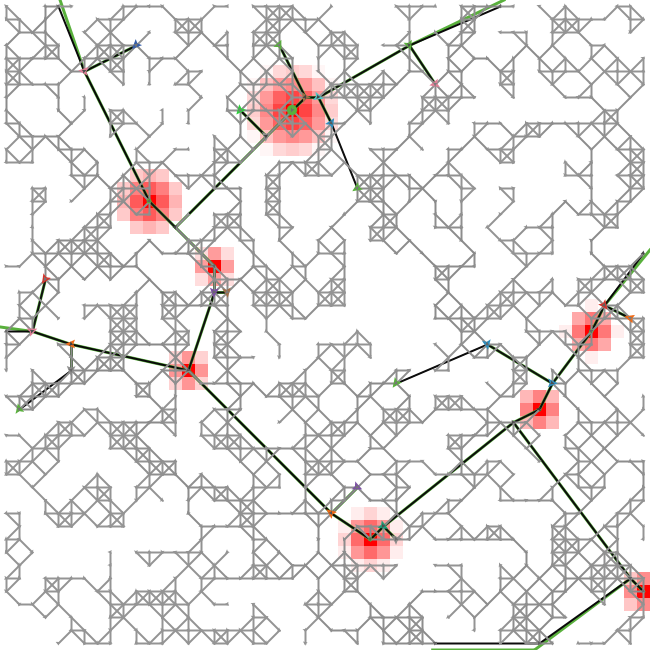
\includegraphics[width=0.48\linewidth]{Figures/NetworkGrowth/example-bio-process-1}}\hspace{0.2cm}
%\frame{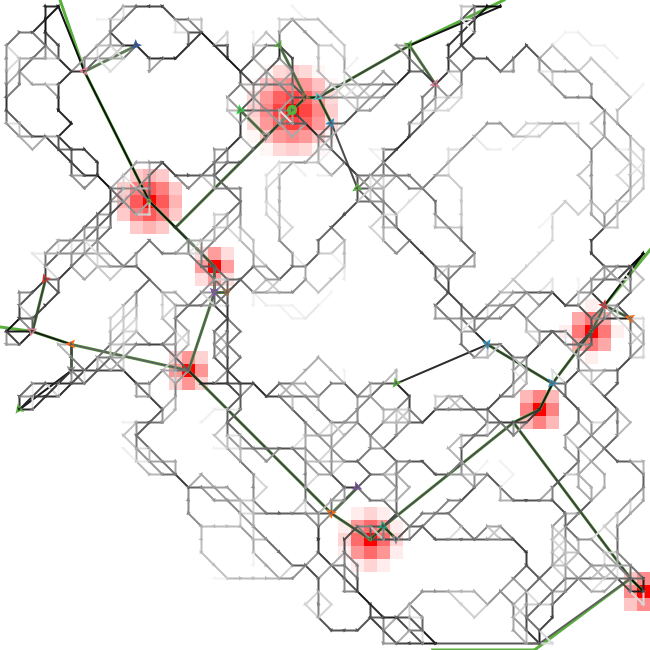
\includegraphics[width=0.48\linewidth]{Figures/NetworkGrowth/example-bio-process-1-tick80}}
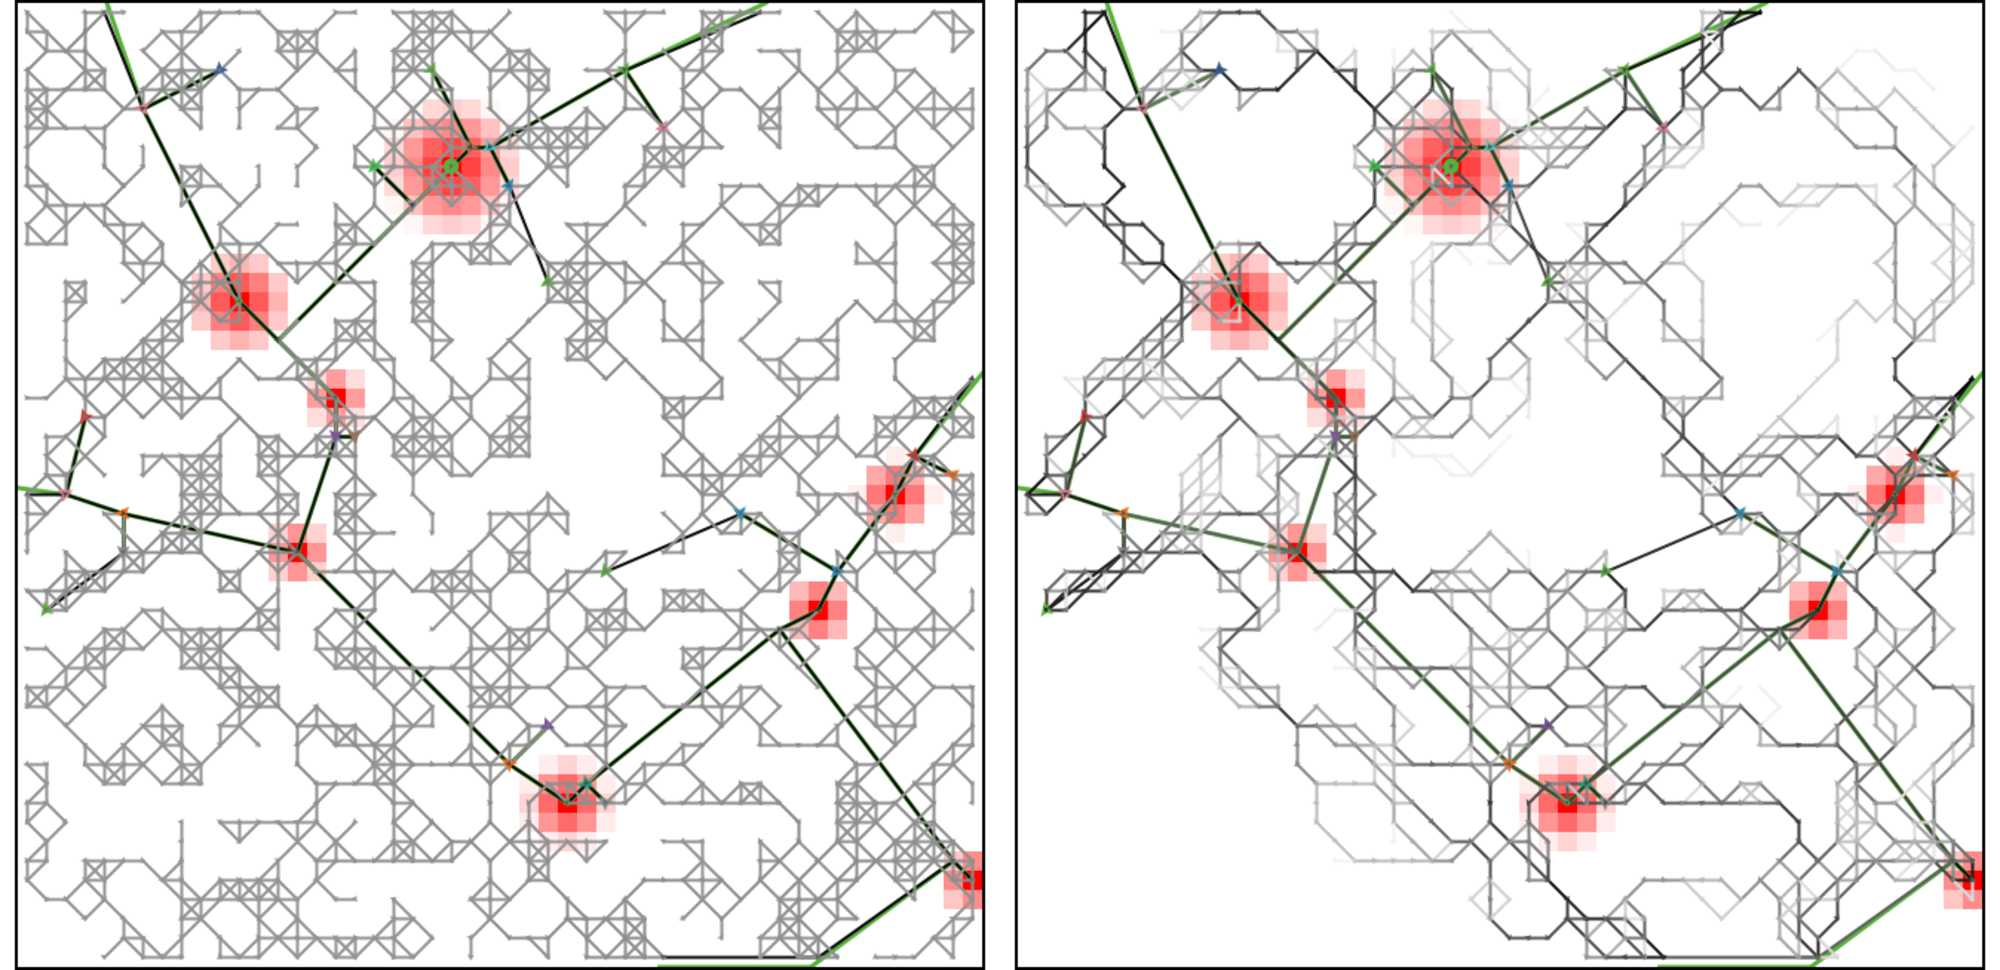
\includegraphics[width=\linewidth]{Figures/Final/7-1-1-fig-networkgrowth-bioexample.jpg}
\caption[Biological network generation example][Exemple de génération de réseau biologique]{\textbf{Biological heuristic for network generation.} This visualization example illustrates the intermediate stages for the addition of links. \textit{(Left)} The initial semi-random network in which the slime-mould is launched; \textit{(Right)} same network after 80 iterations of the slime-mould, the thickness of links giving the capacity.\label{fig:networkgrowth:bioexample}}{\textbf{Heuristique biologique pour la generation de réseau.} Cet exemple de visualisation illustre les étapes intermédiaires pour l'ajout de liens. \textit{(Gauche)} Le réseau semi-aléatoire initial dans lequel le \emph{slime mould} est lancé ; \textit{(Droite)} même réseau après 80 itérations du \emph{slime mould}, l'épaisseur des liens donnant la capacité.\label{fig:networkgrowth:bioexample}}
\end{figure}
%%%%%%%%%%%%%%%%%


%%%%%%%%%%%%%%%%%%%%%%%
\subsubsection{Cost-benefits evaluation}{Evaluation coûts-bénéfices}


\bpar{
The notion of cost is not explicitly included in all the growth heuristics presented up to here - it is implicitly in gravity potentials through the distance decay parameter, and also in the slime-mould since it generates networks exhibiting a compromise between cost and robustness. We therefore add a simple heuristic which is focused on the cost of network links during their extension. It is the heuristic studied by~\cite{louf2013emergence}, which relies on a rationale in transportation economics. Following a logic of cost-benefits analysis by network developments actors, links are sequentially realized for the couple of non-connected cities with a minimal cost, with a cost of the form $d_{ij} - \lambda / V_{ij}$, where the parameter $\lambda$ is the compromise between construction cost and gain in connected potential.
}{
La notion de coût n'est pas présente de manière explicite dans l'ensemble des heuristiques de croissance présentées jusqu'ici - elle l'est de manière implicite dans les potentiels de gravité par le paramètre d'attenuation de la distance, ainsi que dans le \emph{slime-mould} puisque celui-ci génère des réseau compromis entre robustesse et coût. Nous ajoutons donc une heuristique simple qui est centrée sur le coût des tronçons de réseau lors de leur extension. Il s'agit de celle étudiée par~\cite{louf2013emergence}, qui se base sur des arguments d'économie des transports. Suivant une logique d'analyse coûts-bénéfices par les acteurs du développement du réseau, les liens sont réalisés séquentiellement pour les couples de villes non connectées ayant un coût minimal, avec un coût de la forme $d_{ij} - \lambda / V_{ij}$, où le paramètre $\lambda$ est le compromis entre coût de construction et gain de potentiel connecté.
}


% Bien que les problèmes d'évaluation des infrastructures de transport ne puissent se ramener à une simple équation économique unidimensionnelle, des pratiques d'agrégation linéaire coûts-bénéfices, typiques des méthodes de coûts généralisés dont les ingénieurs en transport sont friands, ont été pratiquées pendant un certain temps et le sont encore aujourd'hui dans certain cas. Cet aspect a été intégré dans un modèle de génération de réseau de manière volontairement naïve par~\cite{louf2013emergence}, qui permet déjà de produire un hiérarchie et une transition de phase dans le réseau de transport. Nous proposons de comparer cette heuristique aux autres afin de voir le rôle du coût qui n'est pas présent explicitement dans celles-ci.



%%%%%%%%%%%%%%%%%%%%%%%
\subsubsection{Parameters}{Paramètres}


\bpar{
We summarize the parameters that will vary in the following in Table~\ref{tab:networkgrowth:parameters}. An additional ``parameter'', or more precisely a meta-parameter, is the choice of the heuristic to add links.
}{
Nous résumons les paramètres que nous ferons varier par la suite en Table~\ref{tab:networkgrowth:parameters}. Un ``paramètre'' supplémentaire, ou plutôt un méta-paramètre, est le choix de l'heuristique pour l'ajout des liens.
}


%%%%%%%%%%%%%%
\begin{table}
\caption[Summary of network growth parameters][Résumé des paramètres de croissance de réseau]{\textbf{Summary of network growth parameters for all heuristics.} We also give the corresponding processes, typical variation ranges and their default values.\label{tab:networkgrowth:parameters}}{\textbf{Résumé des paramètres de croissance de réseau pour l'ensemble des heuristiques.} Nous donnons également les processus correspondants, les bornes typiques de variation et leur valeur par défaut.\label{tab:networkgrowth:parameters}}
\bpar{
\begin{tabular}{|c|c|c|c|c|c|}
  \hline
Heuristic & Parameter & Name & Process & Domain & Default\\
  \hline
\multirow{5}{*}{Base}& $l_m$ & added links & growth & $[0;100]$ & $10$ \\\cline{2-6}
 & $d_G$ & gravity distance & potential & $]0;5000]$ & $500$ \\\cline{2-6}
 & $d_0$ & gravity shape & potential & $]0;10]$ & $2$ \\\cline{2-6}
 & $k_h$ & gravity weight & potential & $[0;1]$ & $0.5$ \\\cline{2-6}
 & $\gamma_G$ & gravity hierarchy & potential & $[0.1;4]$ & $1.5$ \\\hline
\multirow{2}{*}{Random breakdown}& $\gamma_R$ & random selection hierarchy & hierarchy & $[0.1;4]$ & $1.5$ \\\cline{2-6}
& $\theta_R$ & random threshold & breakdown & $[1;5]$ & $2$ \\\hline
Cost-benefits & $\lambda$ & compromise & compromise & $[0;0.1]$ & $0.05$ \\\hline
\multirow{2}{*}{Biological}& $n_b$ & iterations & convergence & $[40;100]$ & $50$ \\\cline{2-6}
& $\theta_b$ & biological threshold & threshold & $[0.1;1.0]$ & $0.5$ \\\hline
\end{tabular}
}{
\begin{tabular}{|c|c|c|c|c|c|}
  \hline
Heuristique & Paramètre & Nom & Processus & Domaine & Défaut\\
  \hline
\multirow{5}{*}{Base}& $l_m$ & liens ajoutés & croissance & $[0;100]$ & $10$ \\\cline{2-6}
 & $d_G$ & distance gravitaire & potentiel & $]0;5000]$ & $500$ \\\cline{2-6}
 & $d_0$ & forme gravitaire & potentiel & $]0;10]$ & $2$ \\\cline{2-6}
 & $k_h$ & poids gravitaire & potentiel & $[0;1]$ & $0.5$ \\\cline{2-6}
 & $\gamma_G$ & hiérarchie gravitaire & potentiel & $[0.1;4]$ & $1.5$ \\\hline
\multirow{2}{*}{Rupture aléatoire}& $\gamma_R$ & hiérarchie aléatoire & hiérarchie & $[0.1;4]$ & $1.5$ \\\cline{2-6}
& $\theta_R$ & seuil aléatoire & rupture & $[1;5]$ & $2$ \\\hline
Coût-Bénéfices& $\lambda$ & compromis & compromis & $[0;0.1]$ & $0.05$ \\\hline
\multirow{2}{*}{Biologique}& $n_b$ & itérations & convergence & $[40;100]$ & $50$ \\\cline{2-6}
& $\theta_b$ & seuil biologique & seuil & $[0.1;1.0]$ & $0.5$ \\\hline
\end{tabular}
}
\end{table}
%%%%%%%%%%%%%%






%%%%%%%%%%%%%%%%%%%%%%%
\subsection{Results}{Résultats}


\subsubsection{Model setup}{Initialisation du modèle}

\bpar{
The model is initialized on synthetic or semi-synthetic configurations, with a grid of size $N=50$, with the following steps.
\begin{enumerate}
	\item Population density is initialized either with an exponential mixture, which centers (network nodes) follow the configuration of a synthetic city system as done in~\ref{sec:macrocoevolexplo}; or from a real configuration extracted from the density raster for France. We will use the second option here in systematic explorations.
	\item In the second case, a fixed number of network nodes are generated and located following a preferential attachment to density (see~\ref{sec:correlatedsyntheticdata})\footnote{To avoid bord effects of a network with no connection to the exterior, we add a fixed number $n_e$ of nodes (that we take as $n_e = 6$) at random locations on the border of the world.}. We do not initialize on real networks, since these will be the calibration target, but impose an initial synthetic skeleton that can be interpreted as an archaic network.
	\item An initial network is generated by connecting the nodes as detailed in~\ref{sec:correlatedsyntheticdata}.
\end{enumerate}
}{
Le modèle est initialisé sur configurations synthétiques ou semi-synthétiques, avec une grille de taille $N=50$, selon les étapes suivantes.
\begin{enumerate}
	\item La densité de population est initialisée soit par mélange d'exponentielles, dont les centres (noeuds du réseau) suivent la configuration d'un système de ville synthétique comme fait en~\ref{sec:macrocoevolexplo} ; soit à partir d'une configuration réelle extraite du raster de densité pour la France. Nous utiliserons la deuxième option dans les explorations systématiques ici.
	\item Dans le second cas, un nombre fixe de noeud du réseau sont générés et localisés de manière préférentielle selon la densité (voir~\ref{sec:correlatedsyntheticdata})\footnote{Pour éviter les effets de bord d'un réseau n'ayant aucune connexion avec l'extérieur, nous ajoutons un nombre fixe $n_e$ de noeuds (que nous prenons $n_e = 6$) à des points aléatoires sur le bord du monde.}. Nous n'initialisons pas sur réseau réel puisqu'il s'agira de la cible de calibration, mais imposons un squelette initial synthétique pouvant être interprété comme un réseau archaïque.
	\item Un réseau initial est créé par connection des noeuds comme détaillé en~\ref{sec:correlatedsyntheticdata}.
\end{enumerate}
}


\subsubsection{Generated networks}{Réseaux générés}


\bpar{
A visual illustration of the different generated topologies is given in Fig.~\ref{fig:networkgrowth:examples} for a synthetic density configuration. This allows us to compare the particularities of each heuristic. For example, links formed through random breakdown compared to deterministic breakdown witness the path-dependency and produce a less redundant network, whereas deterministic breakdown reinforces the strongest link between the two large cities that are close. The cost-based heuristic gives network that are dense in a very localized way, but avoids too long links. Finally, the biological heuristic produces a dense mesh in the sub-region where interactions are the strongest.
}{
Une illustration visuelle des différentes topologies générées est donnée en Fig.~\ref{fig:networkgrowth:examples} pour une configuration de densité synthétique. Cela permet de comparer les particularités de chacune des heuristiques. Par exemple, les liens formés par la rupture aléatoire en comparaison à la rupture déterministe témoignent de la dépendance au chemin et produisent un réseau moins redondant, tandis que la rupture déterministe renforce le lien le plus fort entre les deux grandes villes proches. L'heuristique basée sur le coût donne des réseaux denses de manière très localisée, mais évite les liens trop longs. Enfin, l'heuristique biologique produit un maillage dense dans la sous-région où les interactions sont les plus fortes.
}




%%%%%%%%%%%%%%%%%
\begin{figure}
	% example_comp_nwSize200_setup.png
	%\frame{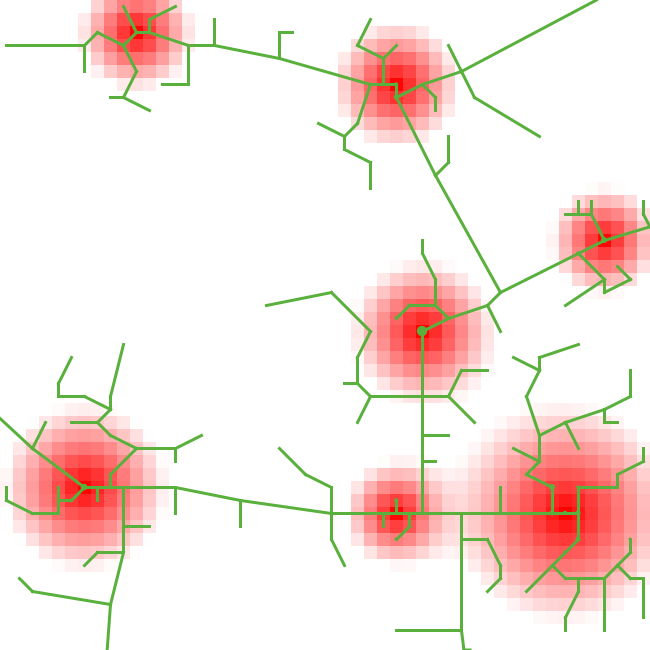
\includegraphics[width=0.32\linewidth]{Figures/NetworkGrowth/example_comp_nwSize200_connex.png}}
	%\frame{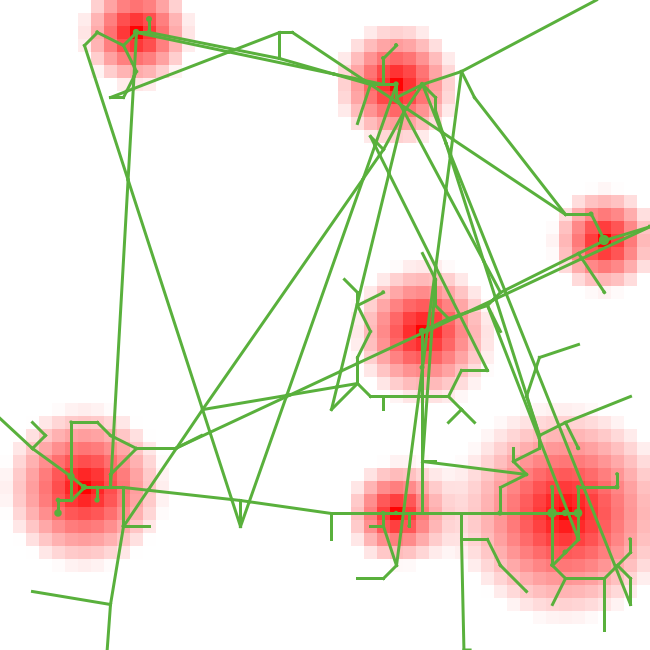
\includegraphics[width=0.32\linewidth]{Figures/NetworkGrowth/example_comp_nwSize200_random.png}}
	%\frame{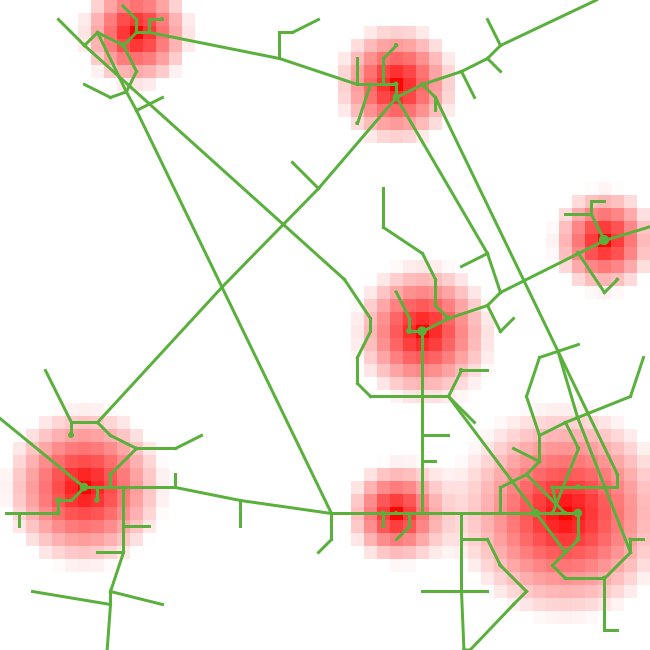
\includegraphics[width=0.32\linewidth]{Figures/NetworkGrowth/example_comp_nwSize200_rndbrkdwn.png}}\\
	%\frame{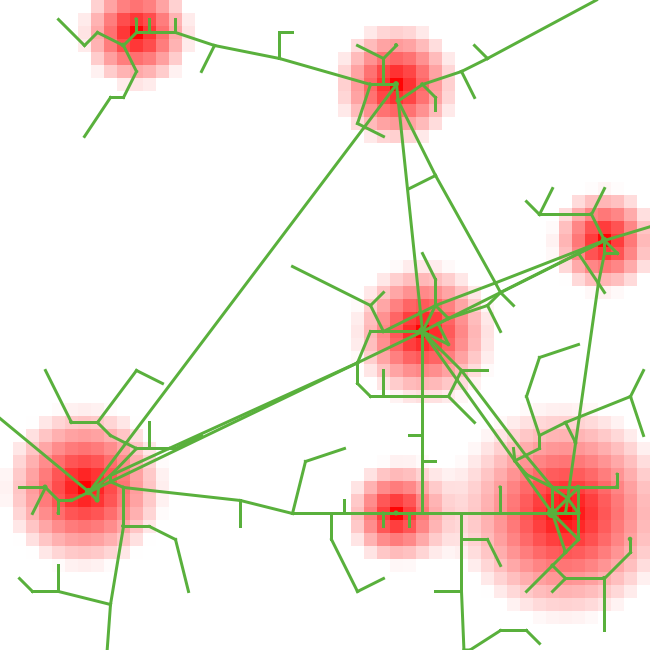
\includegraphics[width=0.32\linewidth]{Figures/NetworkGrowth/example_comp_nwSize200_detbrkdwn.png}}
	%\frame{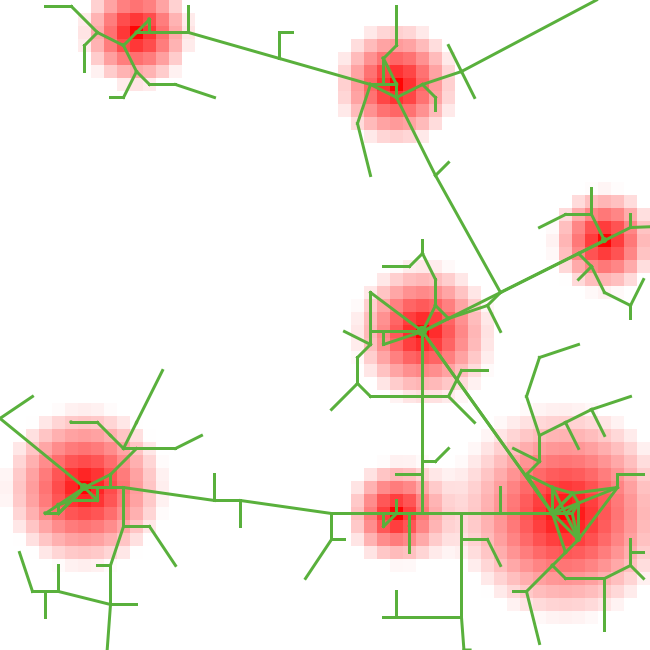
\includegraphics[width=0.32\linewidth]{Figures/NetworkGrowth/example_comp_nwSize200_cost.png}}
	%\frame{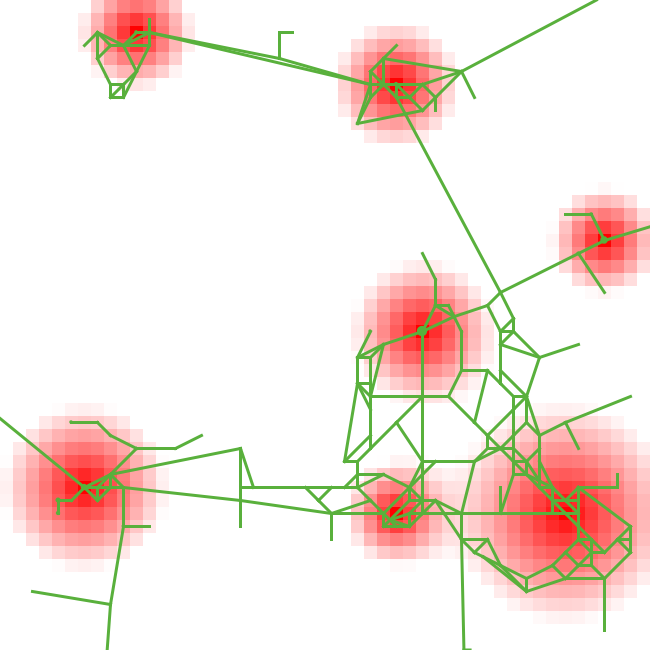
\includegraphics[width=0.32\linewidth]{Figures/NetworkGrowth/example_comp_nwSize200_bio.png}}
	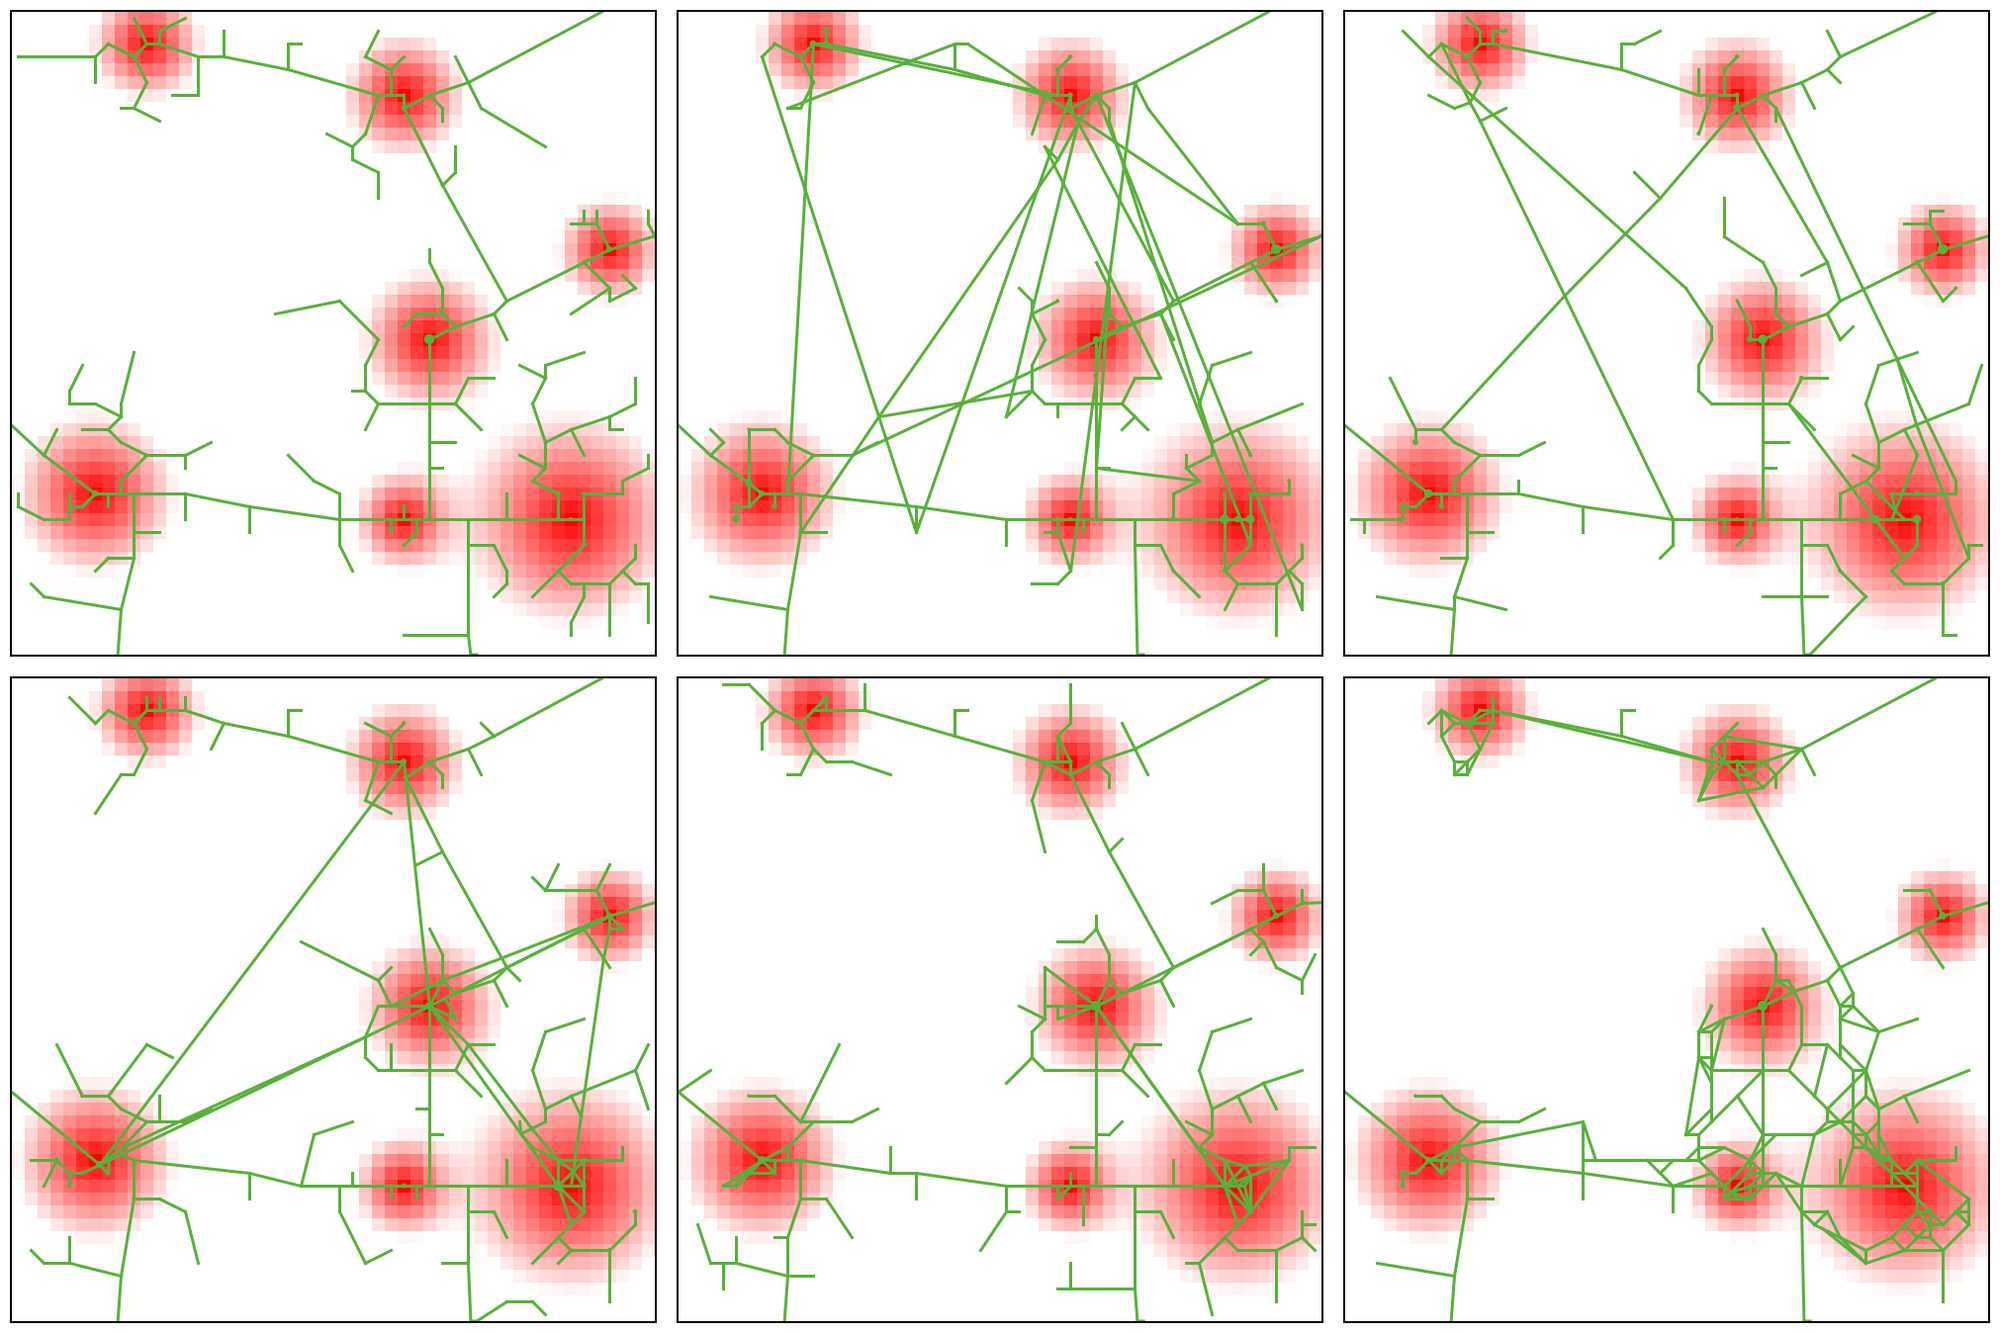
\includegraphics[width=\linewidth]{Figures/Final/7-1-2-fig-networkgrowth-examples.jpg}
\caption[Network examples for different generation heuristics][Exemples de réseaux pour différentes heuristiques de génération]{\textbf{Examples of networks obtained with the different heuristics.} Networks are obtained for the same density configuration composed of 7 centers, and for the same initial network connecting them. We take $l_m = 10$ and fix the final size to 200 nodes. Gravity parameters are $d_G = 2000$, $d_0 = 3$, $\gamma_G = 0.3$, $k_h = 0.6$. In the order from left to right and top to bottom: network with connexion only; random network; random potential breakdown with $\gamma_R = 2$ and $\theta_R = 1.6$; deterministic potential breakdown; cost-benefits with $\lambda = 0.009$; biological with $n_b = 50$ and $\theta_b = 0.6$.\label{fig:networkgrowth:examples}}{\textbf{Exemples de réseaux obtenus par les différentes heuristiques.} Les réseaux sont obtenus pour une même configuration de densité composée de 7 centres, et du même réseau initial les reliant. Nous prenons $l_m = 10$ et fixons la taille finale à 200 noeuds. Les paramètres gravitaires sont $d_G = 2000$, $d_0 = 3$, $\gamma_G = 0.3$, $k_h = 0.6$. Dans l'ordre de gauche à droite et de haut en bas : réseau par connexion seule ; réseau aléatoire ; rupture de potentiel aléatoire avec $\gamma_R = 2$ et $\theta_R = 1.6$ ; rupture de potentiel déterministe ; coût bénéfice avec $\lambda = 0.009$ ; biologique avec $n_b = 50$ et $\theta_b = 0.6$.\label{fig:networkgrowth:examples}}
\end{figure}
%%%%%%%%%%%%%%%%%

% Nous fixons ici $n_N = 100$.



\subsubsection{Experience plan}{Plan d'expérience}


\bpar{
We detail now an experience plan to explore the space of networks generated by the different heuristics. Network generation is done with constant population densities, on real configurations that have been morphologically classified in~\ref{sec:staticcorrelations}. We consider 50 real density grids, corresponding to areas in France, classified into 5 morphological classes. Their description is given in Appendix~\ref{app:sec:networkgrowth}, and show that they cover a set of morphologies spanning to very localized and sparse settlements to polycentric structures, and intermediate configurations.
}{
Détaillons un plan d'expérience pour explorer l'espace des réseaux générés par les différentes heuristiques. La génération de réseau est faite à densité de population constante, sur configurations réelles classifiées morphologiquement en~\ref{sec:staticcorrelations}. Nous considérons 50 grilles réelles de densité, correspondant à des zones en France, classées dans 5 classes morphologiques. La description de celles-ci est donnée en Annexe~\ref{app:sec:networkgrowth}, et montre qu'elle couvrent un ensemble de morphologies allant d'établissements très localisés et dispersés à des structures polycentriques, et des configurations intermédiaires.
}


%       moran  distance   entropy     slope rsquaredslope
%1 0.2324194 0.6580061 0.7590965 0.6202700     0.8673209
%2 0.4748752 0.5024231 0.7516852 0.5305178     0.8307633
%3 0.2133188 0.4208907 0.5745856 0.6520814     0.8107935
%4 0.2354844 0.7482191 0.8994017 0.8677689     0.7508533
%5 0.1505684 0.7604514 0.8418746 0.7168180     0.8796809


\bpar{
Given the parameter ranges previously given for each heuristic, we compare the feasible space for a basic exploration with a Latin Hypercube Sampling of parameter space, for all density grids, with 5 repetitions for each parameter point\footnote{What corresponds to around 240000 repetitions of the model. The simulation data is available at \url{http://dx.doi.org/10.7910/DVN/OBQ4CS}.}.
}{
Étant donné les plages de paramètres données précédemment pour chacune des heuristiques, nous comparons l'espace faisable pour une exploration basique en criblage LHS de l'espace des paramètres, pour l'ensemble des grilles de densité, avec 5 répétitions par point de paramètre\footnote{Correspondant à environ 240000 répétitions du modèle. Le jeu de données issu des simulations est disponible à \url{http://dx.doi.org/10.7910/DVN/OBQ4CS}.}.
}

% NOTE : here would be much more useful to do a PSE (for the feasible space part, not for the calibration part)


\subsubsection{Obtained topologies}{Topologies obtenues}


\bpar{
Networks are characterized here with the following indicators: average betweenness centrality $\bar{bw}$ and average closeness centrality $\bar{cl}$, diameter $r$, average path length $\bar{l}$, relative speed $v_0$. To visualize feasible spaces and then compare them to real networks, we reduce the space in a principal hyperplan, from points obtained in simulations. The first two components can be interpreted the following way\footnote{Their composition is given by: $PC1 = - 0.51 \bar{bw} - 0.45 \bar{l} + 0.57 v_0 - 0.43 r + 0.05 \bar{cl}$ and $PC2 = -0.45 \bar{bw} + 0.17 \bar{l} +0.33 v_0 + 0.8 r +0.1 \bar{cl}$.}: the first will characterize networks in which paths are shorter, whereas the second corresponds to networks with a higher average distance, thus more spread in space, but more efficient.
}{
Les réseaux sont caractérisés ici par les indicateurs suivants : centralité de chemin moyenne $\bar{bw}$ et centralité de proximité moyenne $\bar{cl}$, diamètre $r$, longueur moyenne de chemin $\bar{l}$, vitesse relative $v_0$. Pour visualiser les espaces faisables et les comparer aux réseaux réels par la suite, nous réduisons l'espace dans un hyperplan principal, à partir des points obtenus dans les simulations. Les deux premières composantes s'interprètent de la façon suivante\footnote{Leur composition est donnée par : $PC1 = - 0.51 \bar{bw} - 0.45 \bar{l} + 0.57 v_0 - 0.43 r + 0.05 \bar{cl}$ et $PC2 = -0.45 \bar{bw} + 0.17 \bar{l} +0.33 v_0 + 0.8 r +0.1 \bar{cl}$.} : la première va caractériser des réseaux où les chemins sont courts, tandis que la deuxième exprime des réseaux à distance moyenne plus grande, donc plus étalés, mais plus efficients. 
}
 
\bpar{
The point cloud of the topological feasible space, obtained with the experience plan described above, is given in Fig.~\ref{fig:networkgrowth:feasiblespace}. The coverage is allowed by the complementarity of different clouds for each heuristic. For example, the random heuristic is at the total opposite of the reference heuristic along the first component: the reference tree network logically induces a larger number of detours, and thus longer paths. Random breakdown allows to cover a large span of $PC1$ and corresponds more to low values of $PC2$. 
}{
Le nuage de points de l'espace topologique faisable, obtenu avec le plan d'expérience décrit ci-dessus, est donné en Fig.~\ref{fig:networkgrowth:feasiblespace}. La couverture est permise par la complémentarité des différents nuages pour chaque heuristique. Par exemple, l'heuristique aléatoire est à l'opposée complète de l'heuristique de référence le long de la première composante : le réseau arborescent de référence induit logiquement un plus grand nombre de détours, et donc des chemins plus longs. La rupture aléatoire permet de couvrir une grande plage sur $PC1$ et occupe une place privilégiée pour les faibles valeurs de $PC2$.
}



%summary(gnres$concentration)
%   Min. 1st Qu.  Median    Mean 3rd Qu.    Max. 
% 0.3288  0.5383  0.7551  0.7405  1.0000  1.0000 
% 0.85^2+0.15^2 = 0.745
% 0.65^2+0.35^2 = 0.545


\bpar{
To better understand the complementarity of approaches, we can quantify the intersection of point clouds in Fig.~\ref{fig:networkgrowth:feasiblespace} with a simple method: by dividing the plan into a grid (that we take of size 20x20), the proportions $p_{ij}$ of points for each heuristic $j$ for each cell $i$ can be aggregated into a concentration index $h_i = \sum_j p_{ij}^2$ (Herfindhal index) which distribution describes the balance between heuristics in the different regions of space. We obtain for cells a first quartile at $0.54$, a median at $0.76$ and a third quartile at $1$. For comparison, in the case of two types of points only, a repartition 65-35\% gives an index of $0.55$ and a repartition 85-15\% an index of $0.75$, what means that at least half of cells have more than three quarters of points in a unique category. This confirms the conclusion of a strong complementarity of heuristics.
}{
Pour mieux comprendre la complémentarité des approches, nous pouvons quantifier l'intersection des nuages de points de la Fig.~\ref{fig:networkgrowth:feasiblespace} par une méthode simple : en divisant le plan en une grille (qu'on prend de taille 20x20), les proportions $p_{ij}$ de points de chaque heuristique $j$ pour chaque cellule $i$ peuvent être agrégées en un indice de concentration $h_i = \sum_j p_{ij}^2$ (indice de Herfindhal) dont la distribution décrit les équilibres entre heuristiques dans les régions de l'espace. Nous obtenons pour les cellules un premier quartile à $0.54$, une médiane à $0.76$ et un troisième quartile à $1$. Pour comparaison, dans le cas de deux types de points seulement, une répartition 65-35\% donne un indice de $0.55$ et une répartition 85-15\% un indice de $0.75$, ce qui veut dire qu'au moins la moitié des cellules ont plus de trois quarts de points dans une unique catégorie. Cela confirme la conclusion de forte complémentarité des heuristiques.
}



%%%%%%%%%%%%%%%%%
\begin{figure}
%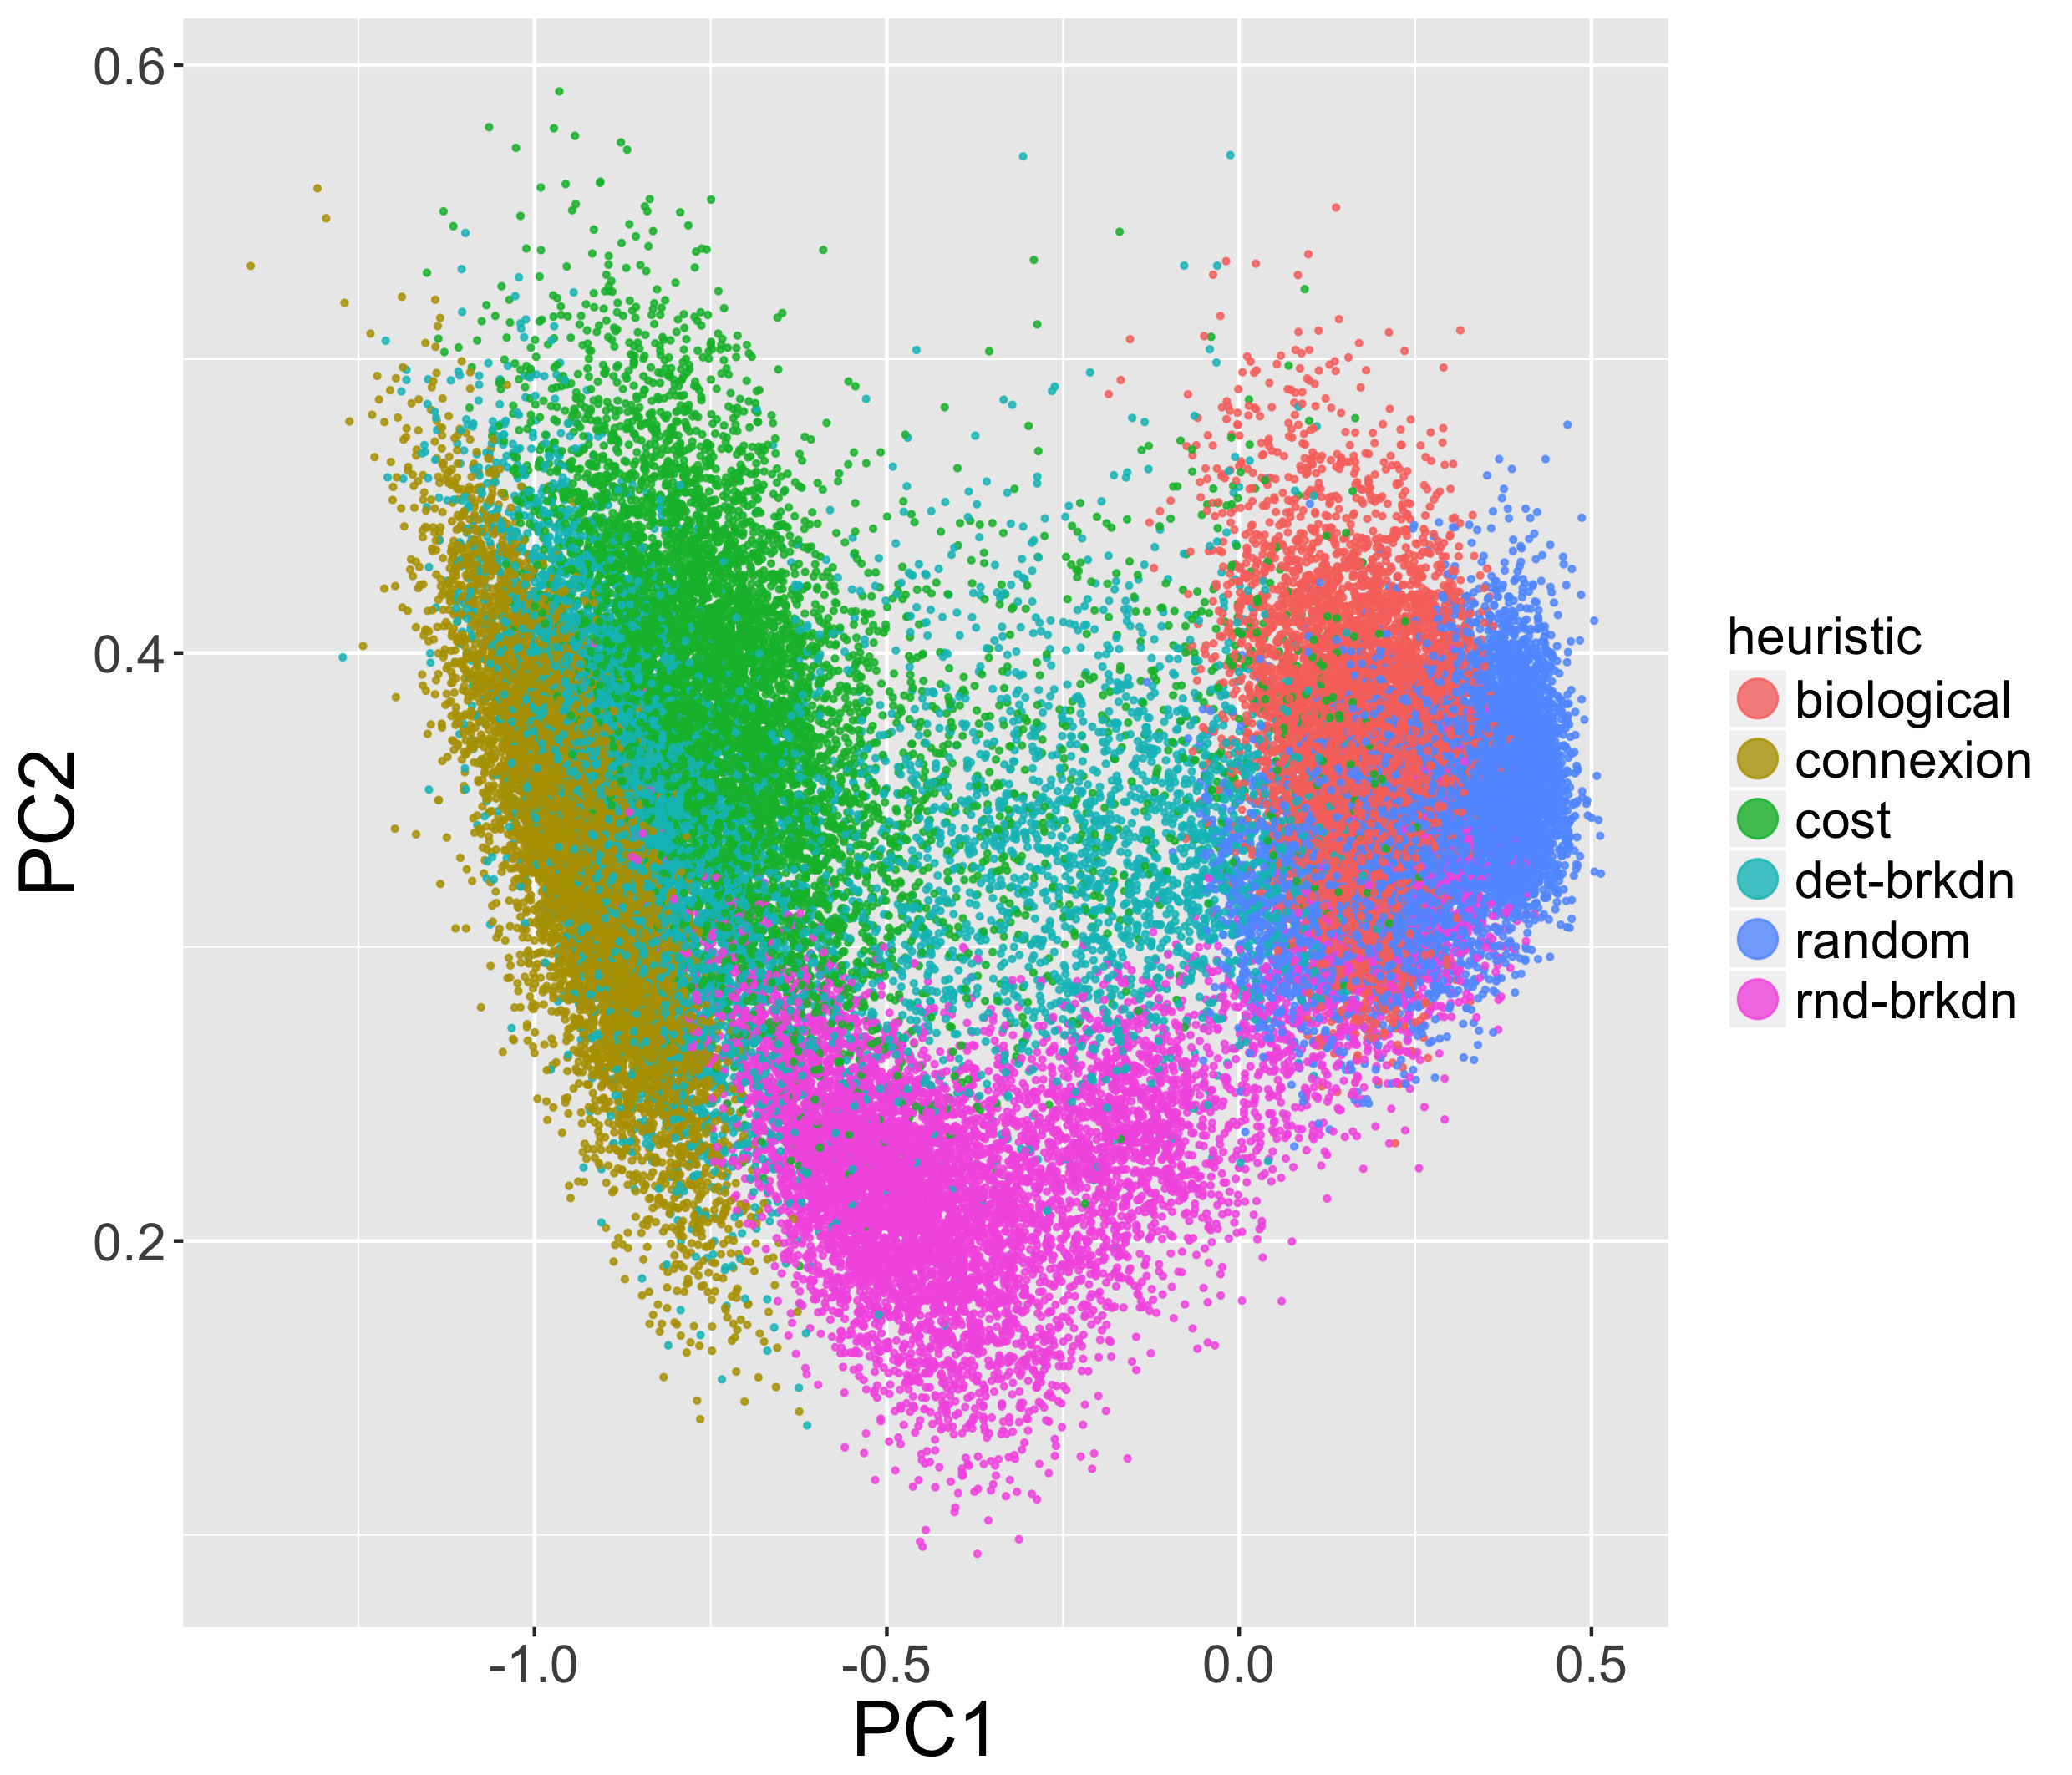
\includegraphics[width=\linewidth]{Figures/NetworkGrowth/feasible_space_pca}
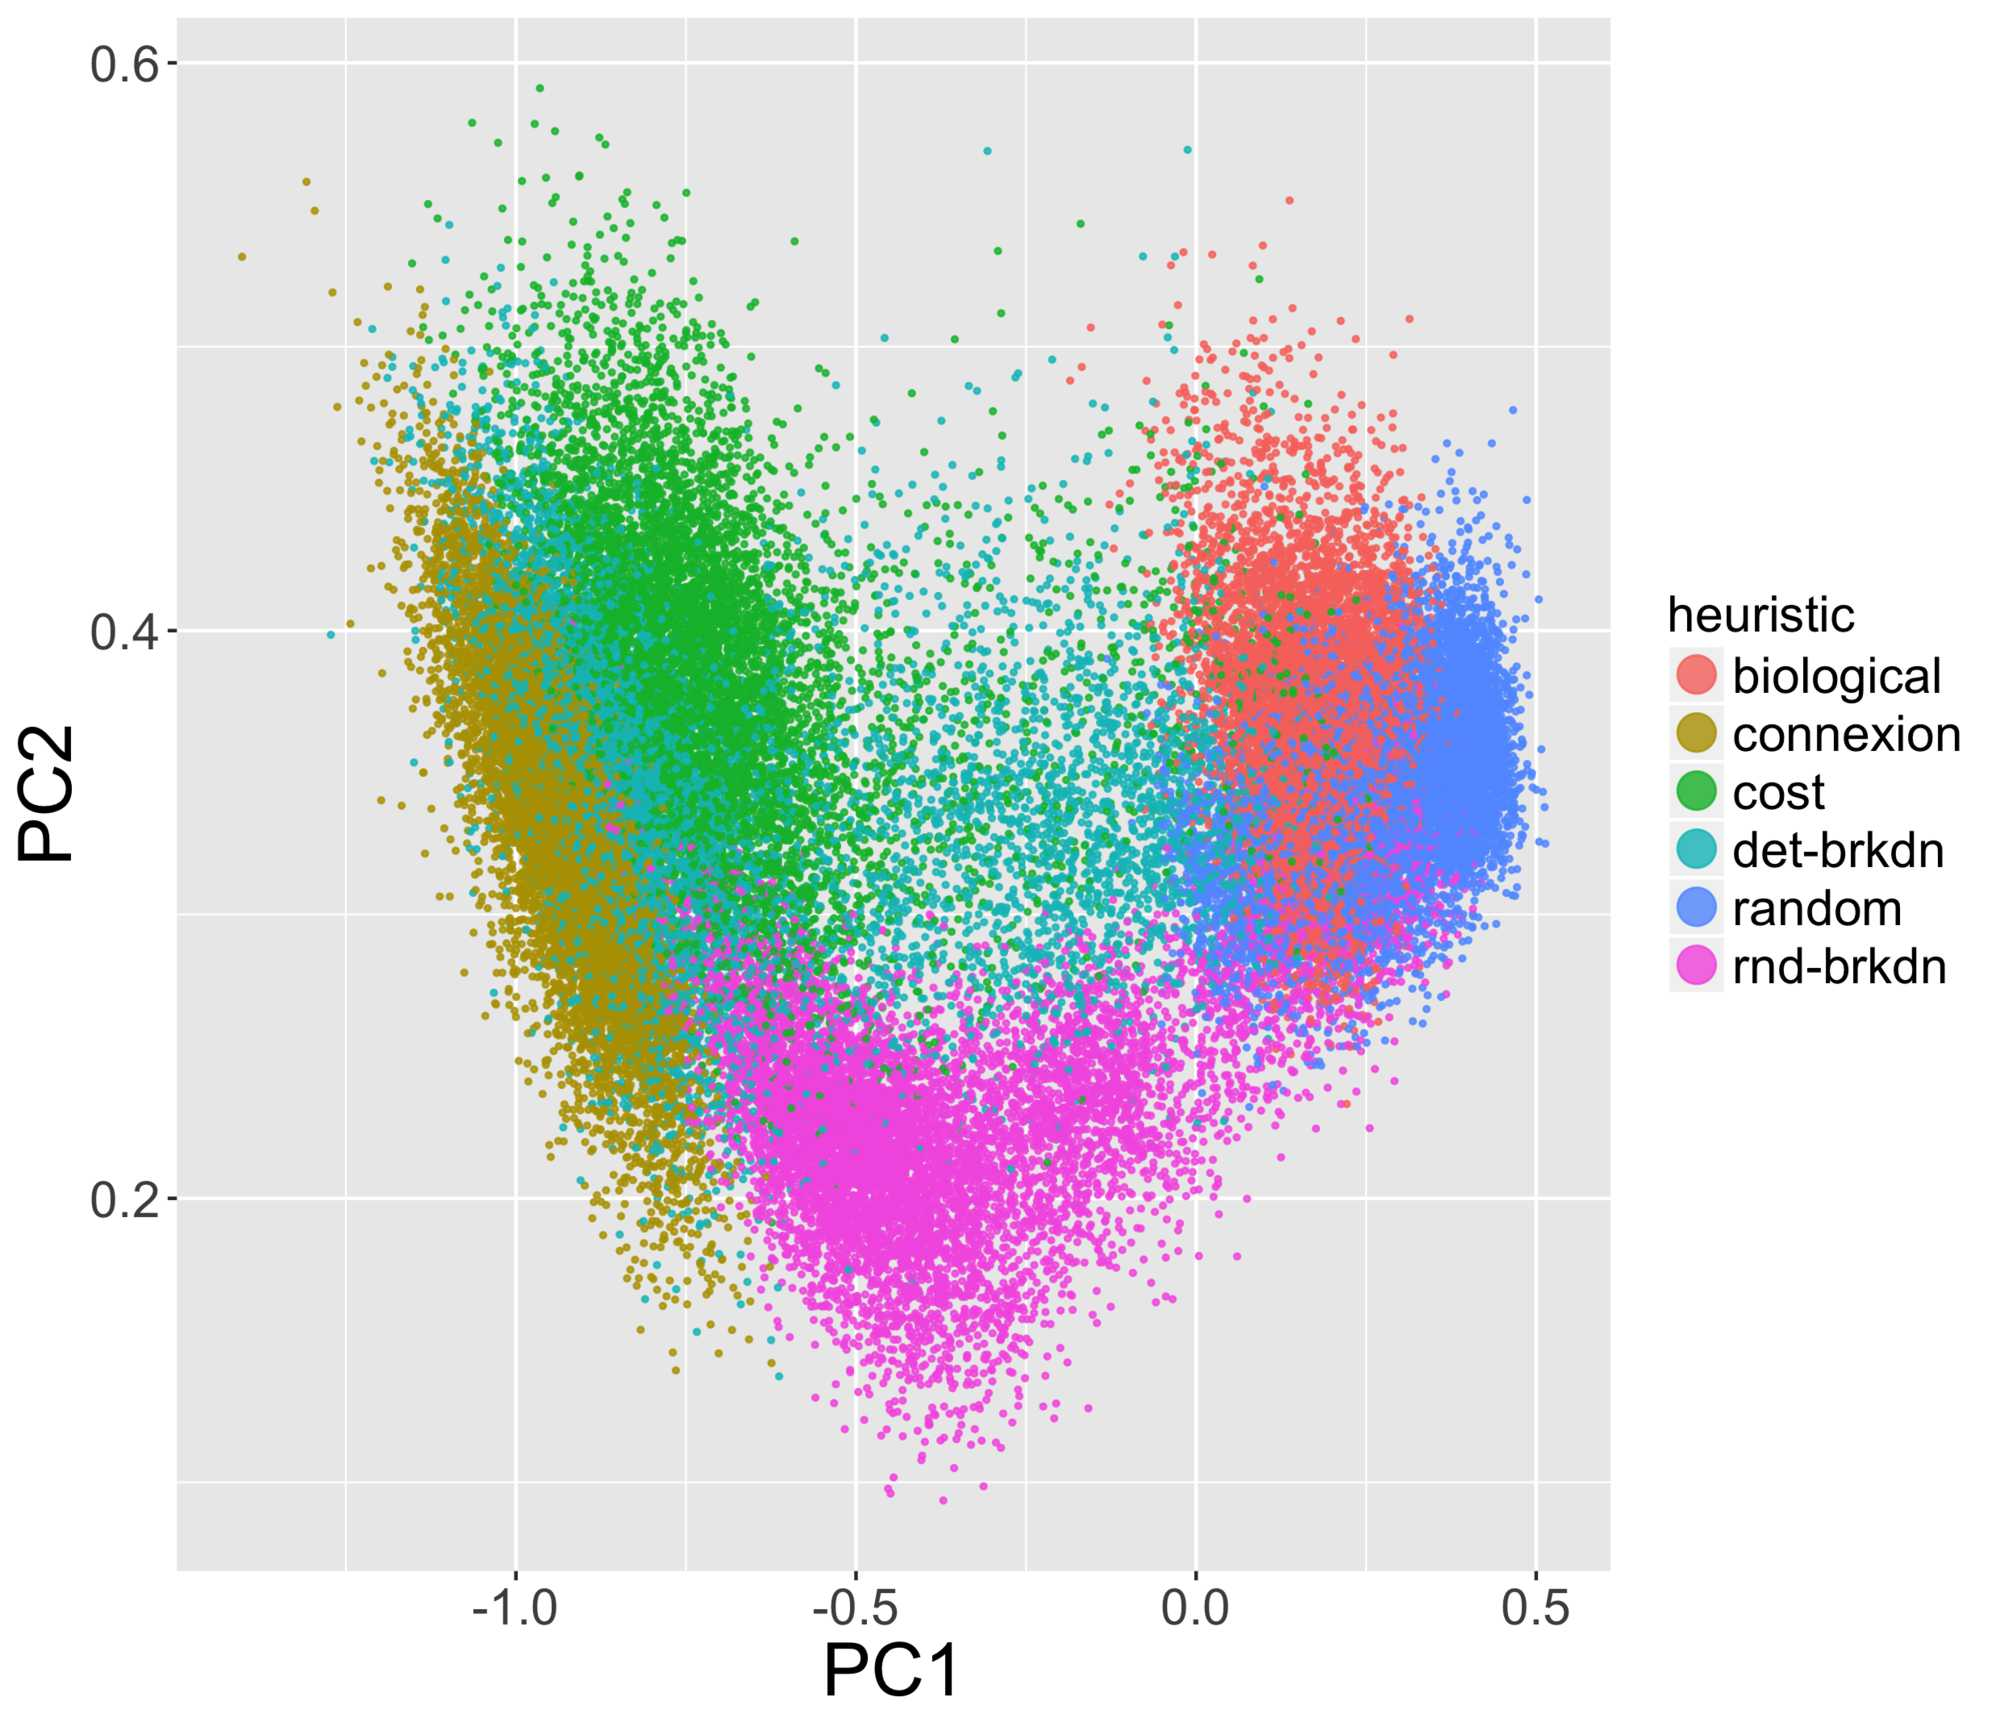
\includegraphics[width=\linewidth]{Figures/Final/7-1-2-fig-networkgrowth-feasiblespace.jpg}
\caption[Feasible topological space][Espace topologique faisable]{\textbf{Feasible topological space for the different generation heuristics.} Point clouds cover complementary regions of the topological space, the color giving the heuristic: biological (\texttt{biological}), reference (\texttt{connexion}), cost-benefits (\texttt{cost}), deterministic breakdown (\texttt{det-brkdn}), random (\texttt{random}) and random breakdown (\texttt{rnd-brkdn}). The same figure conditioned to the morphological class for density is given in Appendix~\ref{app:sec:networkgrowth}.\label{fig:networkgrowth:feasiblespace}}{\textbf{Espace topologique faisable pour les différentes heuristiques de génération.} Les nuages de points couvrent des régions complémentaires de l'espace topologique, la couleur donnant l'heuristique : biologique (\texttt{biological}), référence (\texttt{connexion}), coûts-bénéfices (\texttt{cost}), rupture déterministe (\texttt{det-brkdn}), aléatoire (\texttt{random}) et rupture aléatoire (\texttt{rnd-brkdn}). La même figure conditionnée à la classe morphologique de densité est donnée en Appendice~\ref{app:sec:networkgrowth}.\label{fig:networkgrowth:feasiblespace}}
\end{figure}
%%%%%%%%%%%%%%%%%

% PCA synth
%
%                                PC1        PC2        PC3        PC4         PC5
%meanBwCentrality        -0.51420330 -0.4500671  0.5415210 -0.4602950  0.16708710
%meanPathLength          -0.45662839  0.1782617 -0.2556133  0.3151101  0.77141477
%meanRelativeSpeed        0.57854267  0.3344679  0.3147784 -0.4083421  0.53627500
%nwDiameter              -0.43570261  0.8011179  0.1305644 -0.2508956 -0.29728372
%meanClosenessCentrality  0.05036956  0.1095611  0.7247651  0.6776003 -0.03213514
%Importance of components:
%                          PC1     PC2     PC3     PC4     PC5
%Standard deviation     0.4981 0.06762 0.04611 0.03423 0.02982
%Proportion of Variance 0.9659 0.01780 0.00828 0.00456 0.00346
%Cumulative Proportion  0.9659 0.98370 0.99198 0.99654 1.00000



\subsubsection{Comparison to real networks}{Comparaison aux réseaux réels}

%%%%%%%%%%%%%%%%%
\begin{figure}
%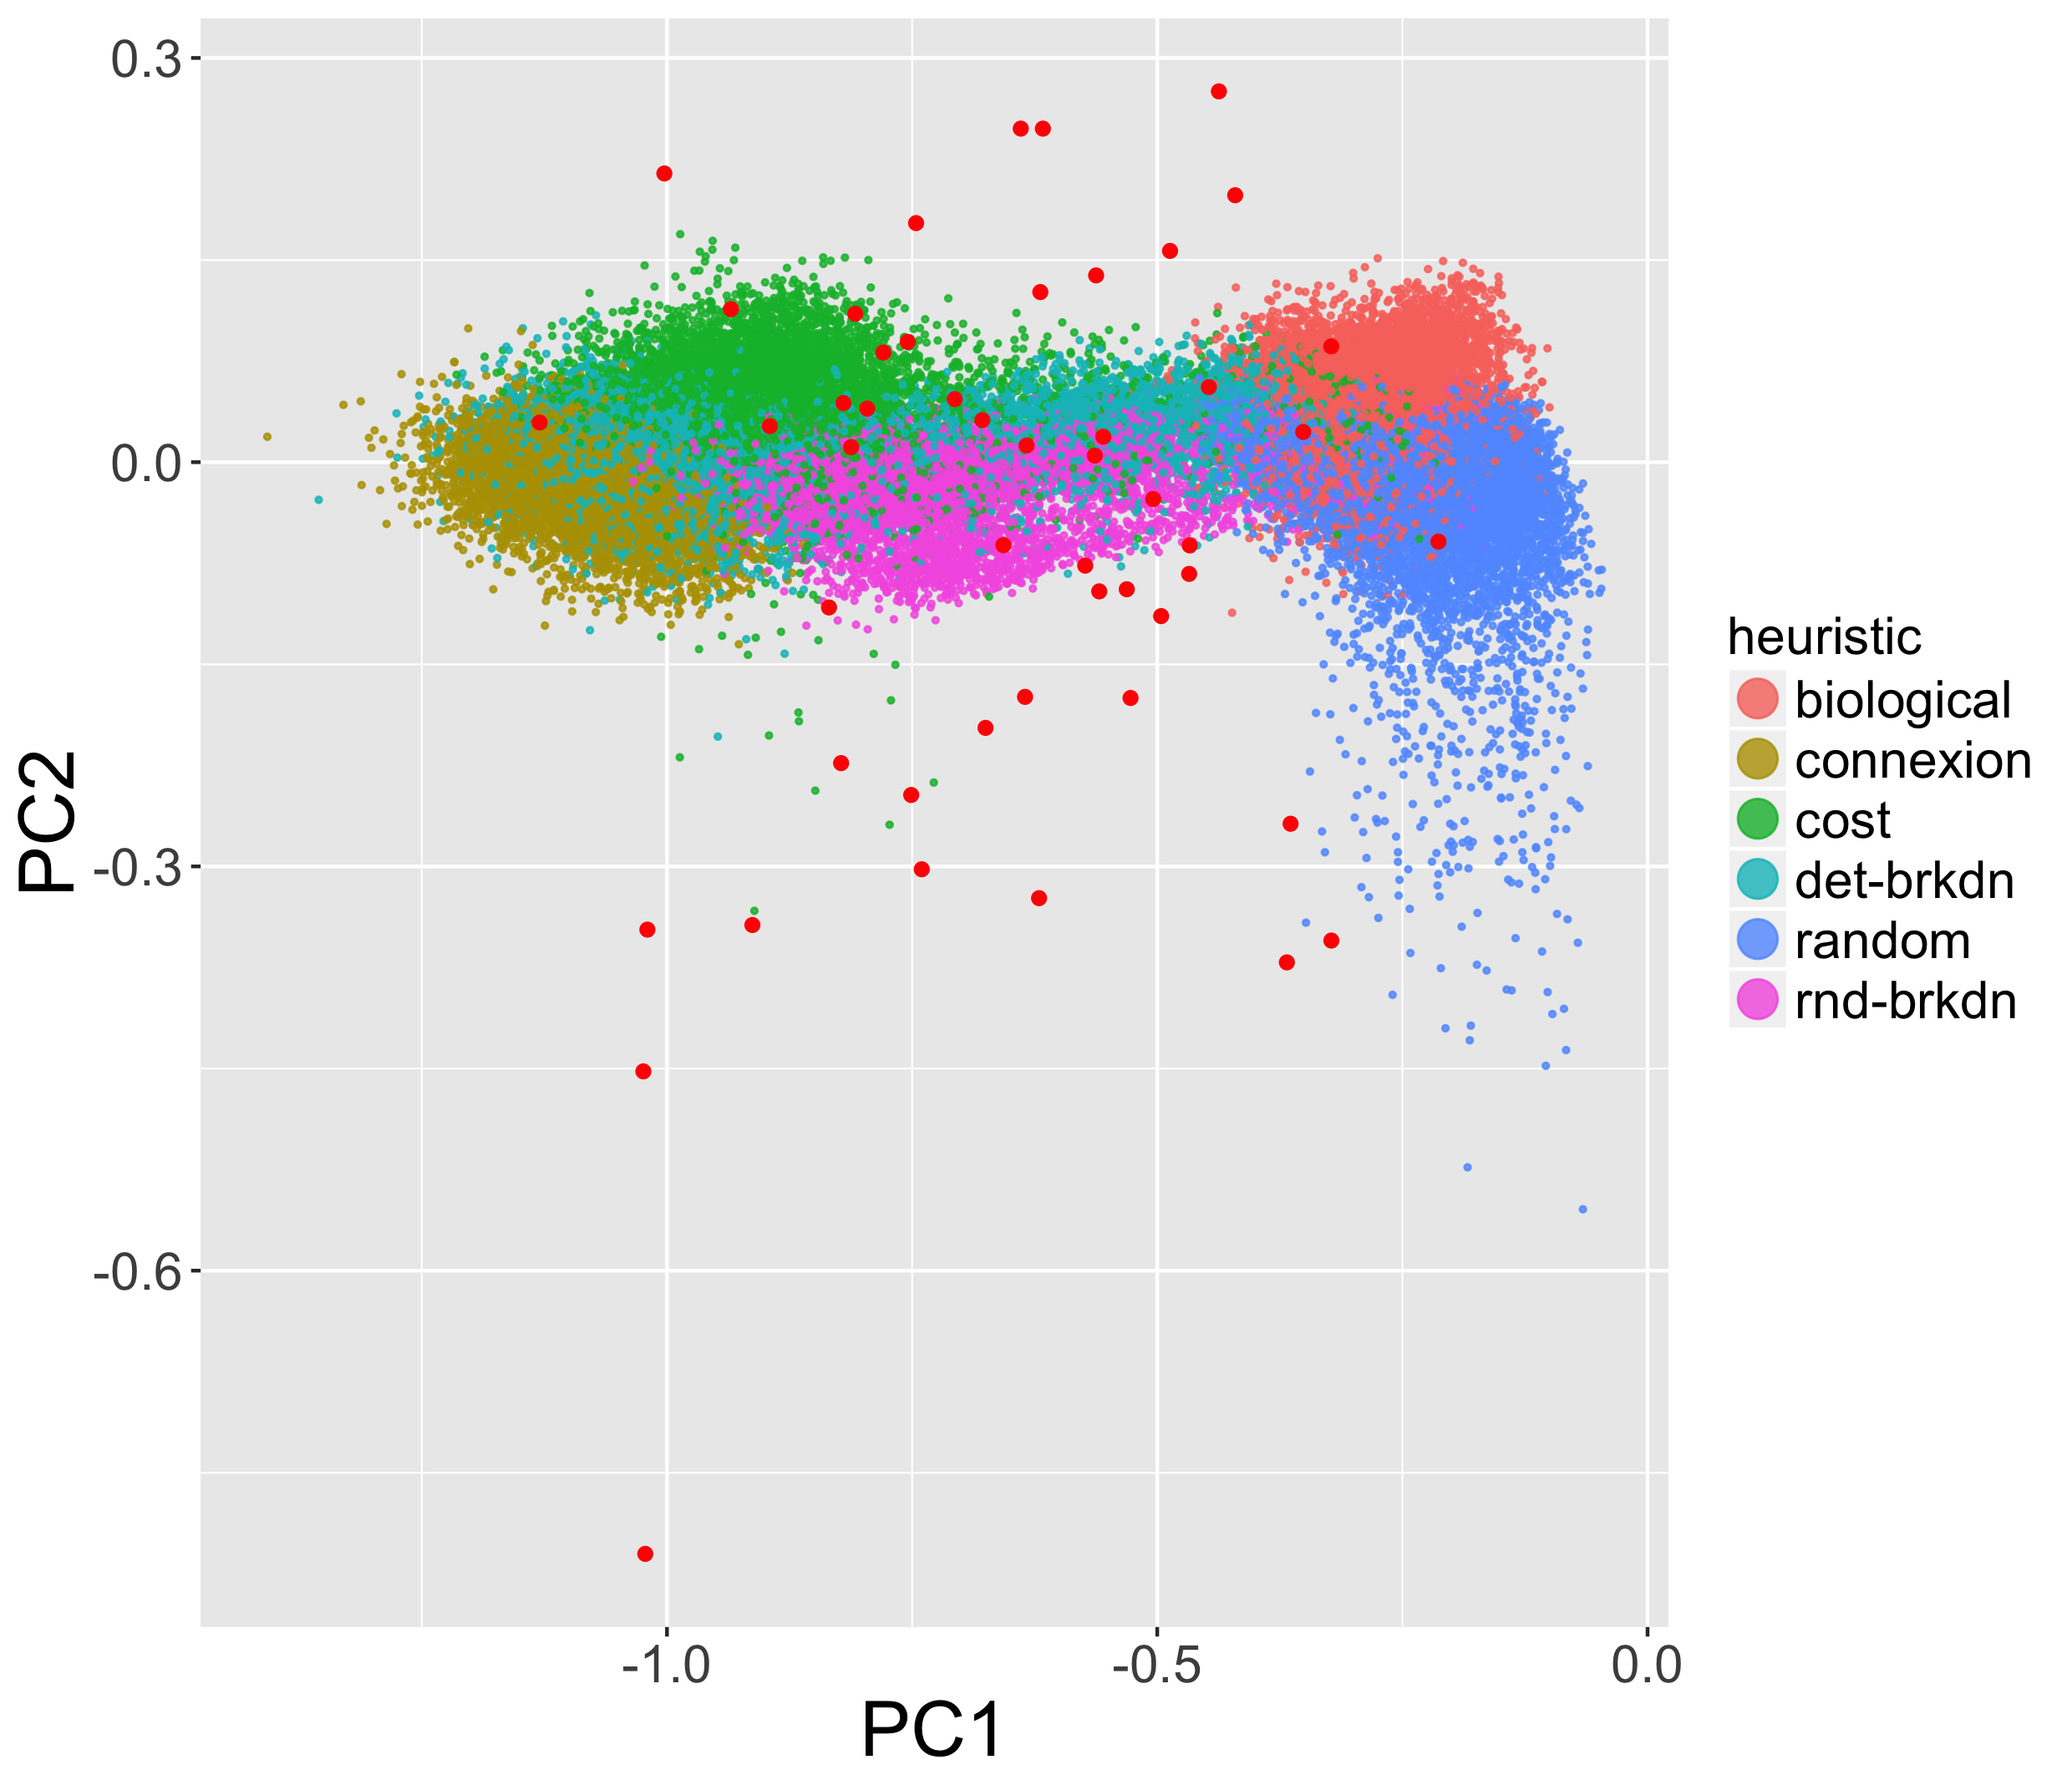
\includegraphics[width=0.45\linewidth]{Figures/NetworkGrowth/feasible_space_withreal_pca}
%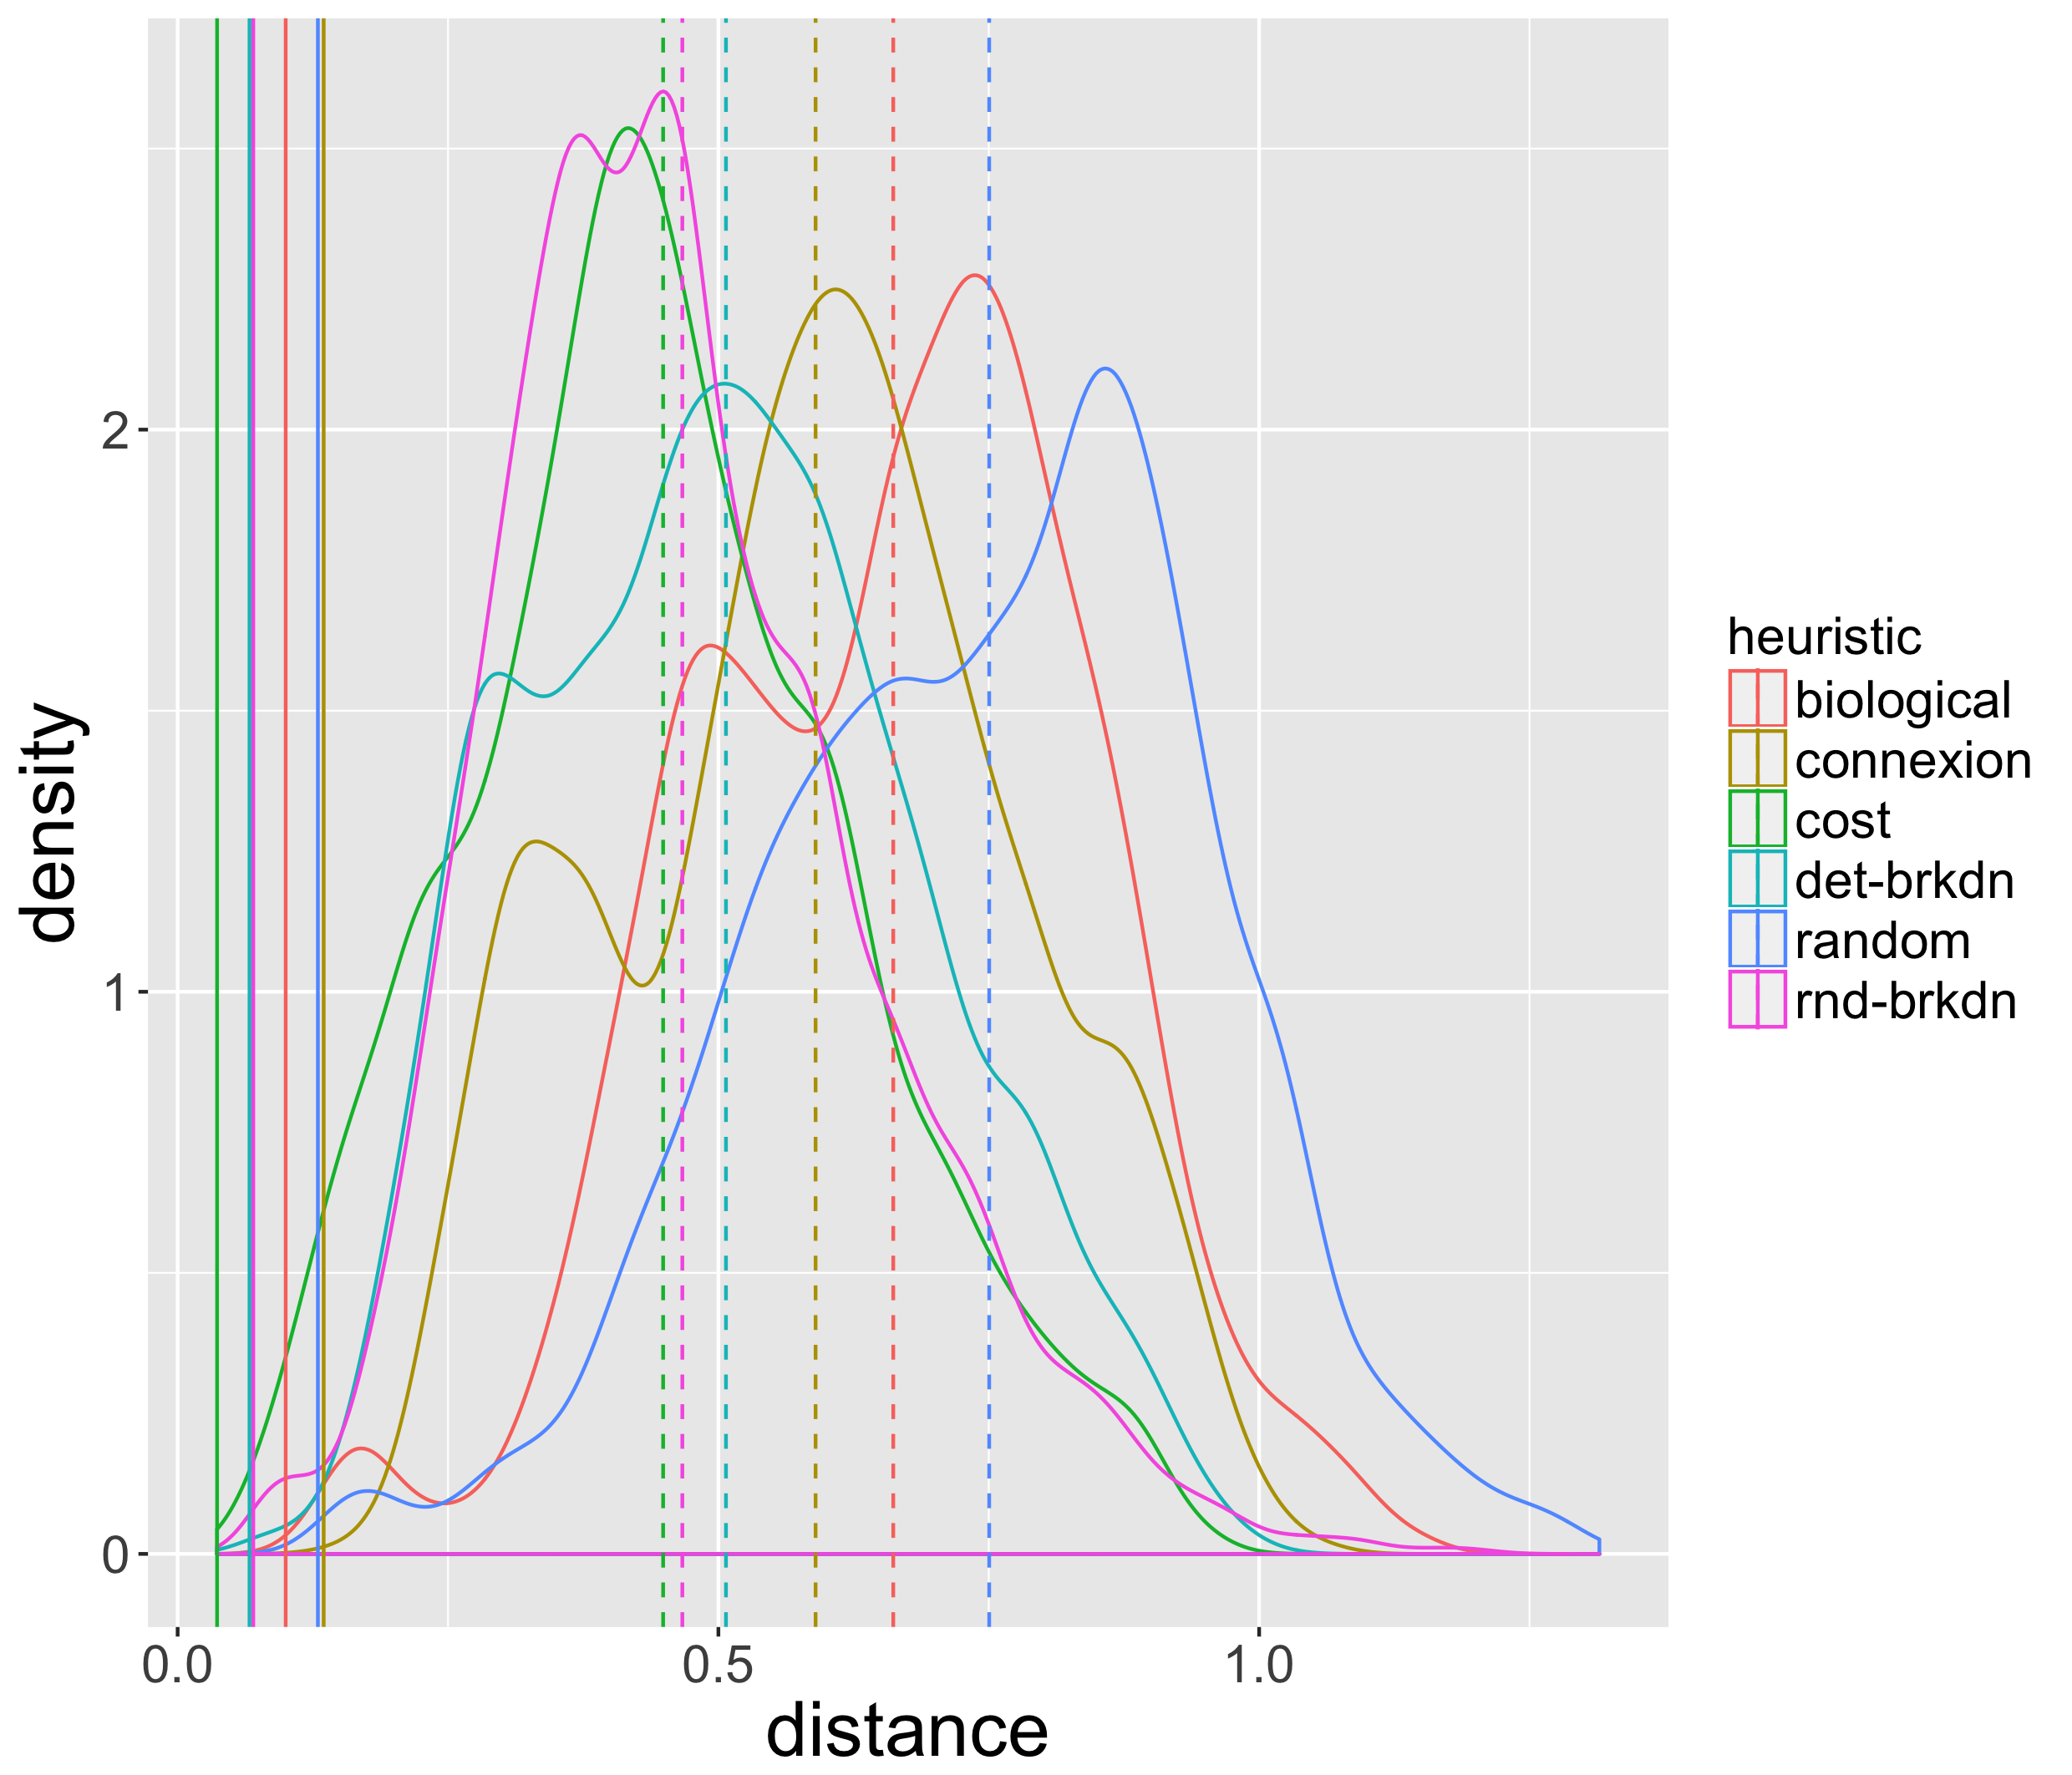
\includegraphics[width=0.45\linewidth]{Figures/NetworkGrowth/distance_real}\\
%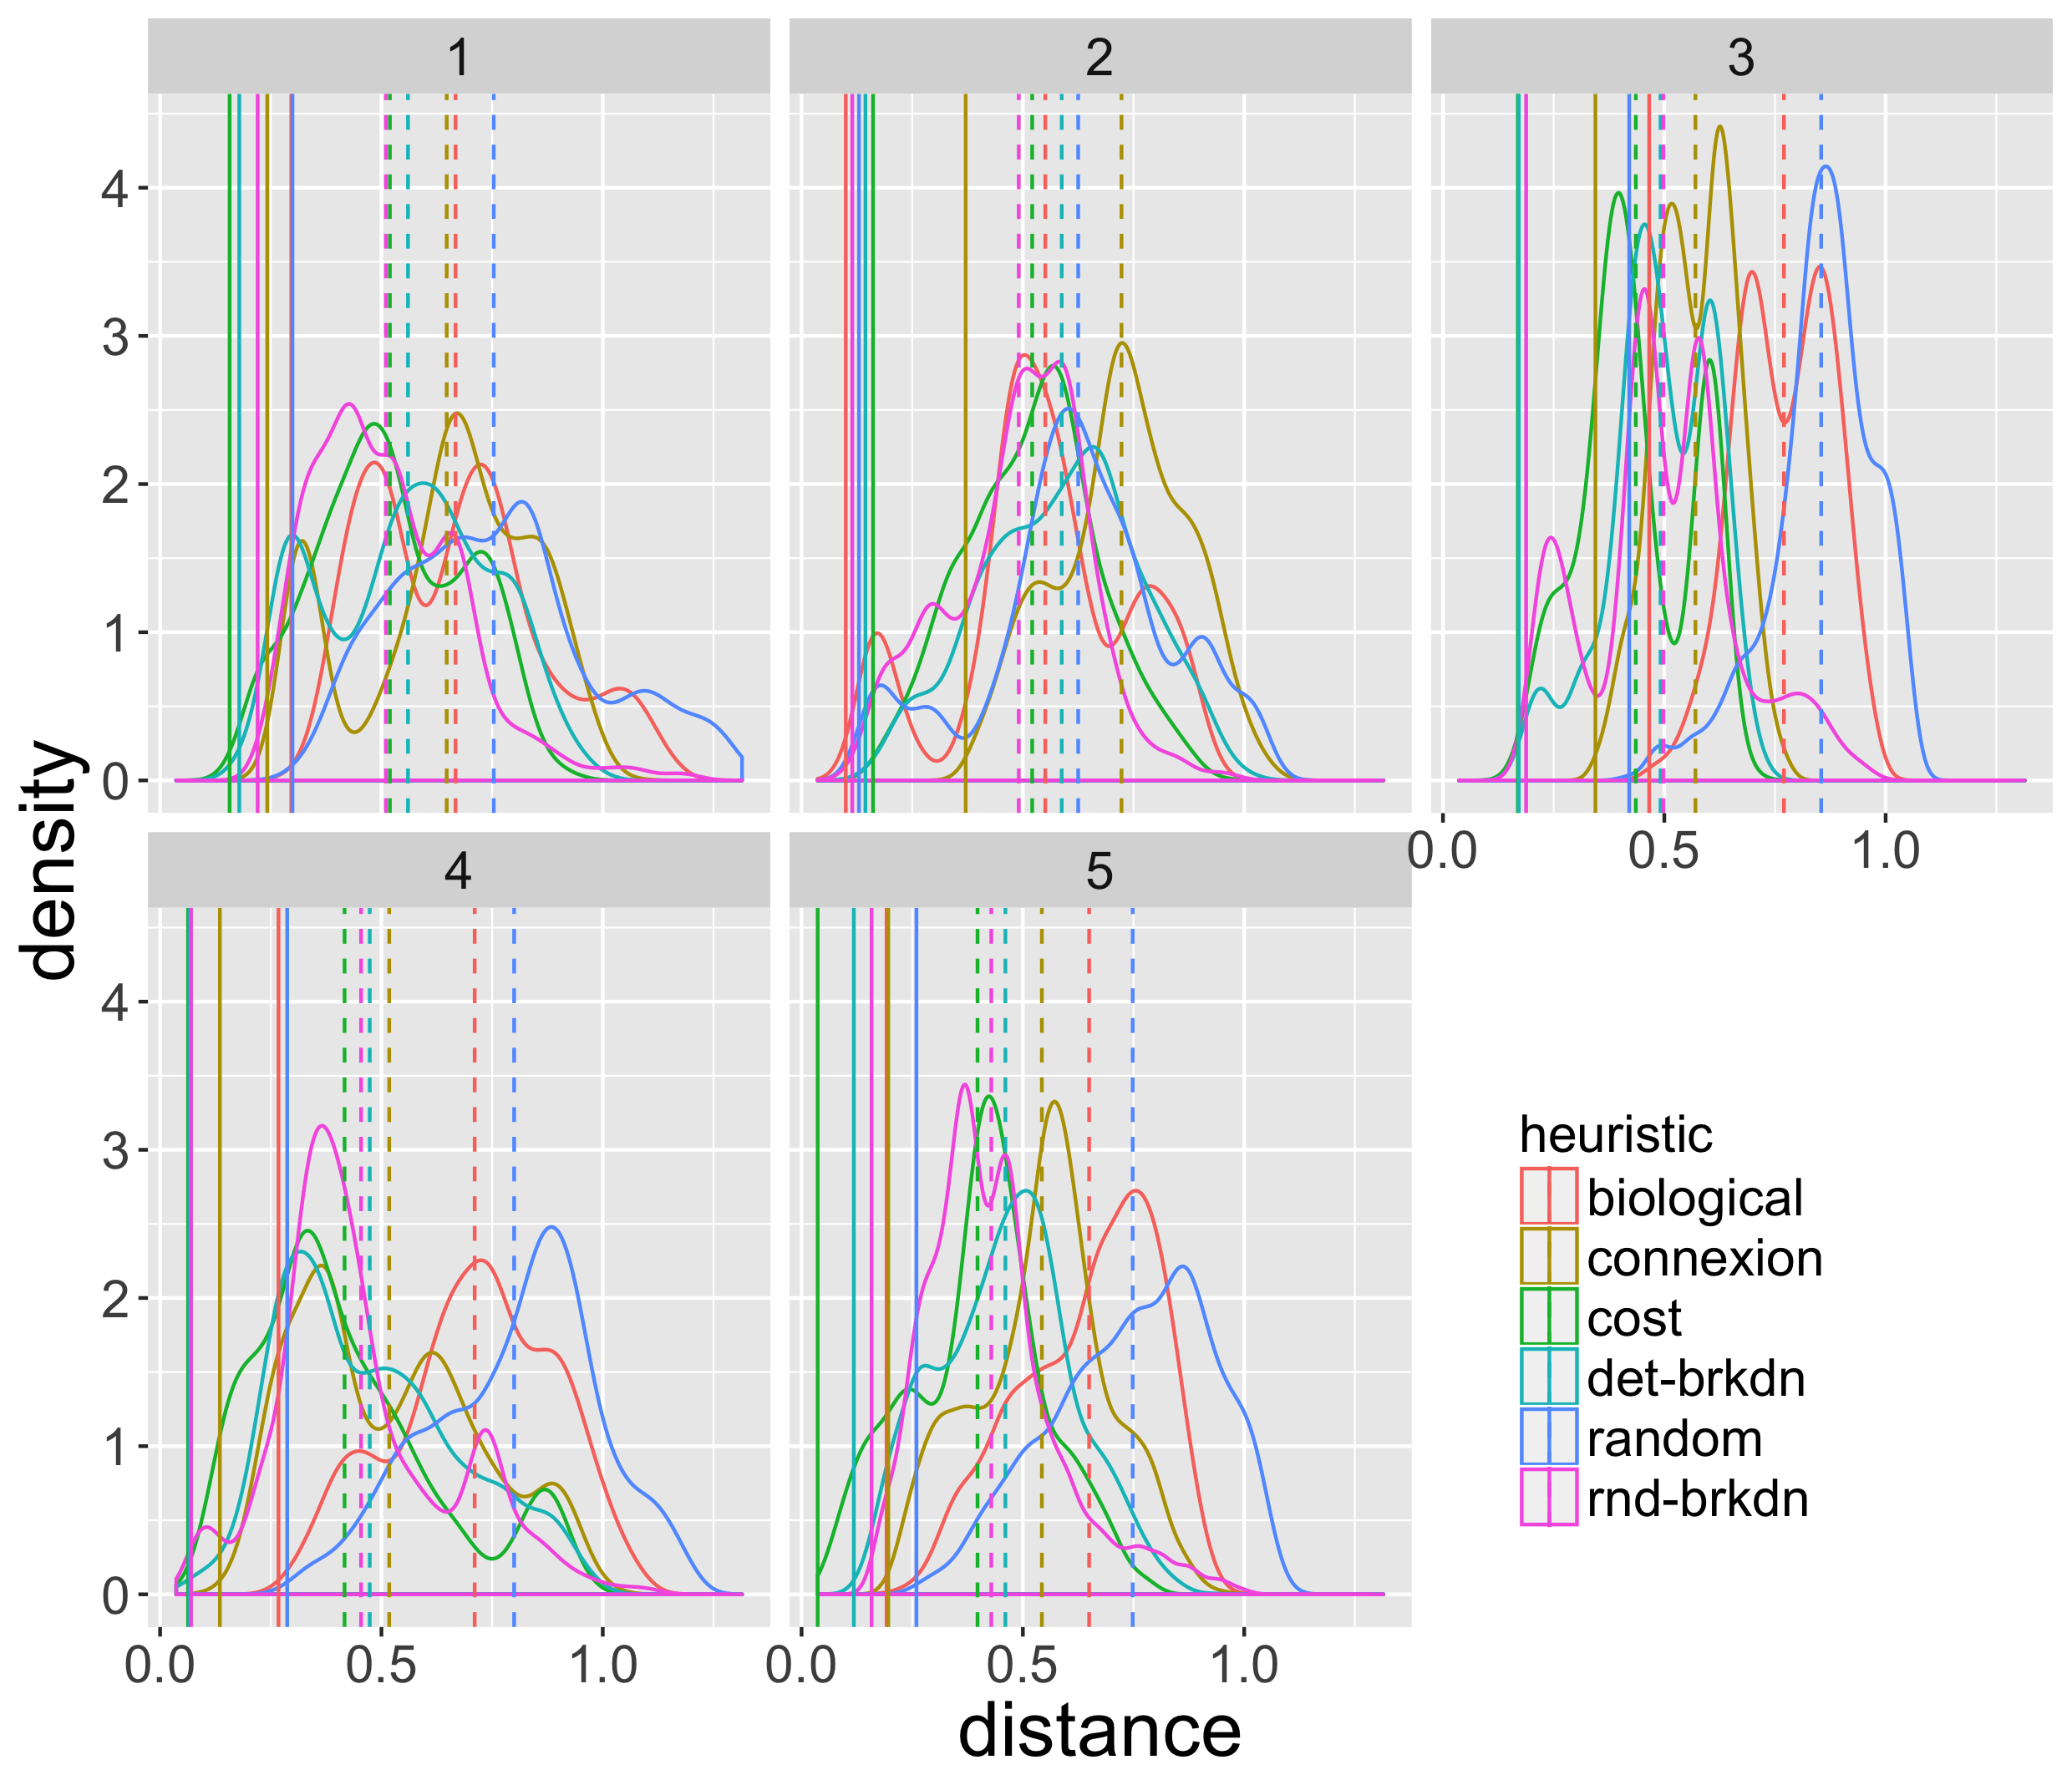
\includegraphics[width=0.8\linewidth]{Figures/NetworkGrowth/distance_real_bymorph}
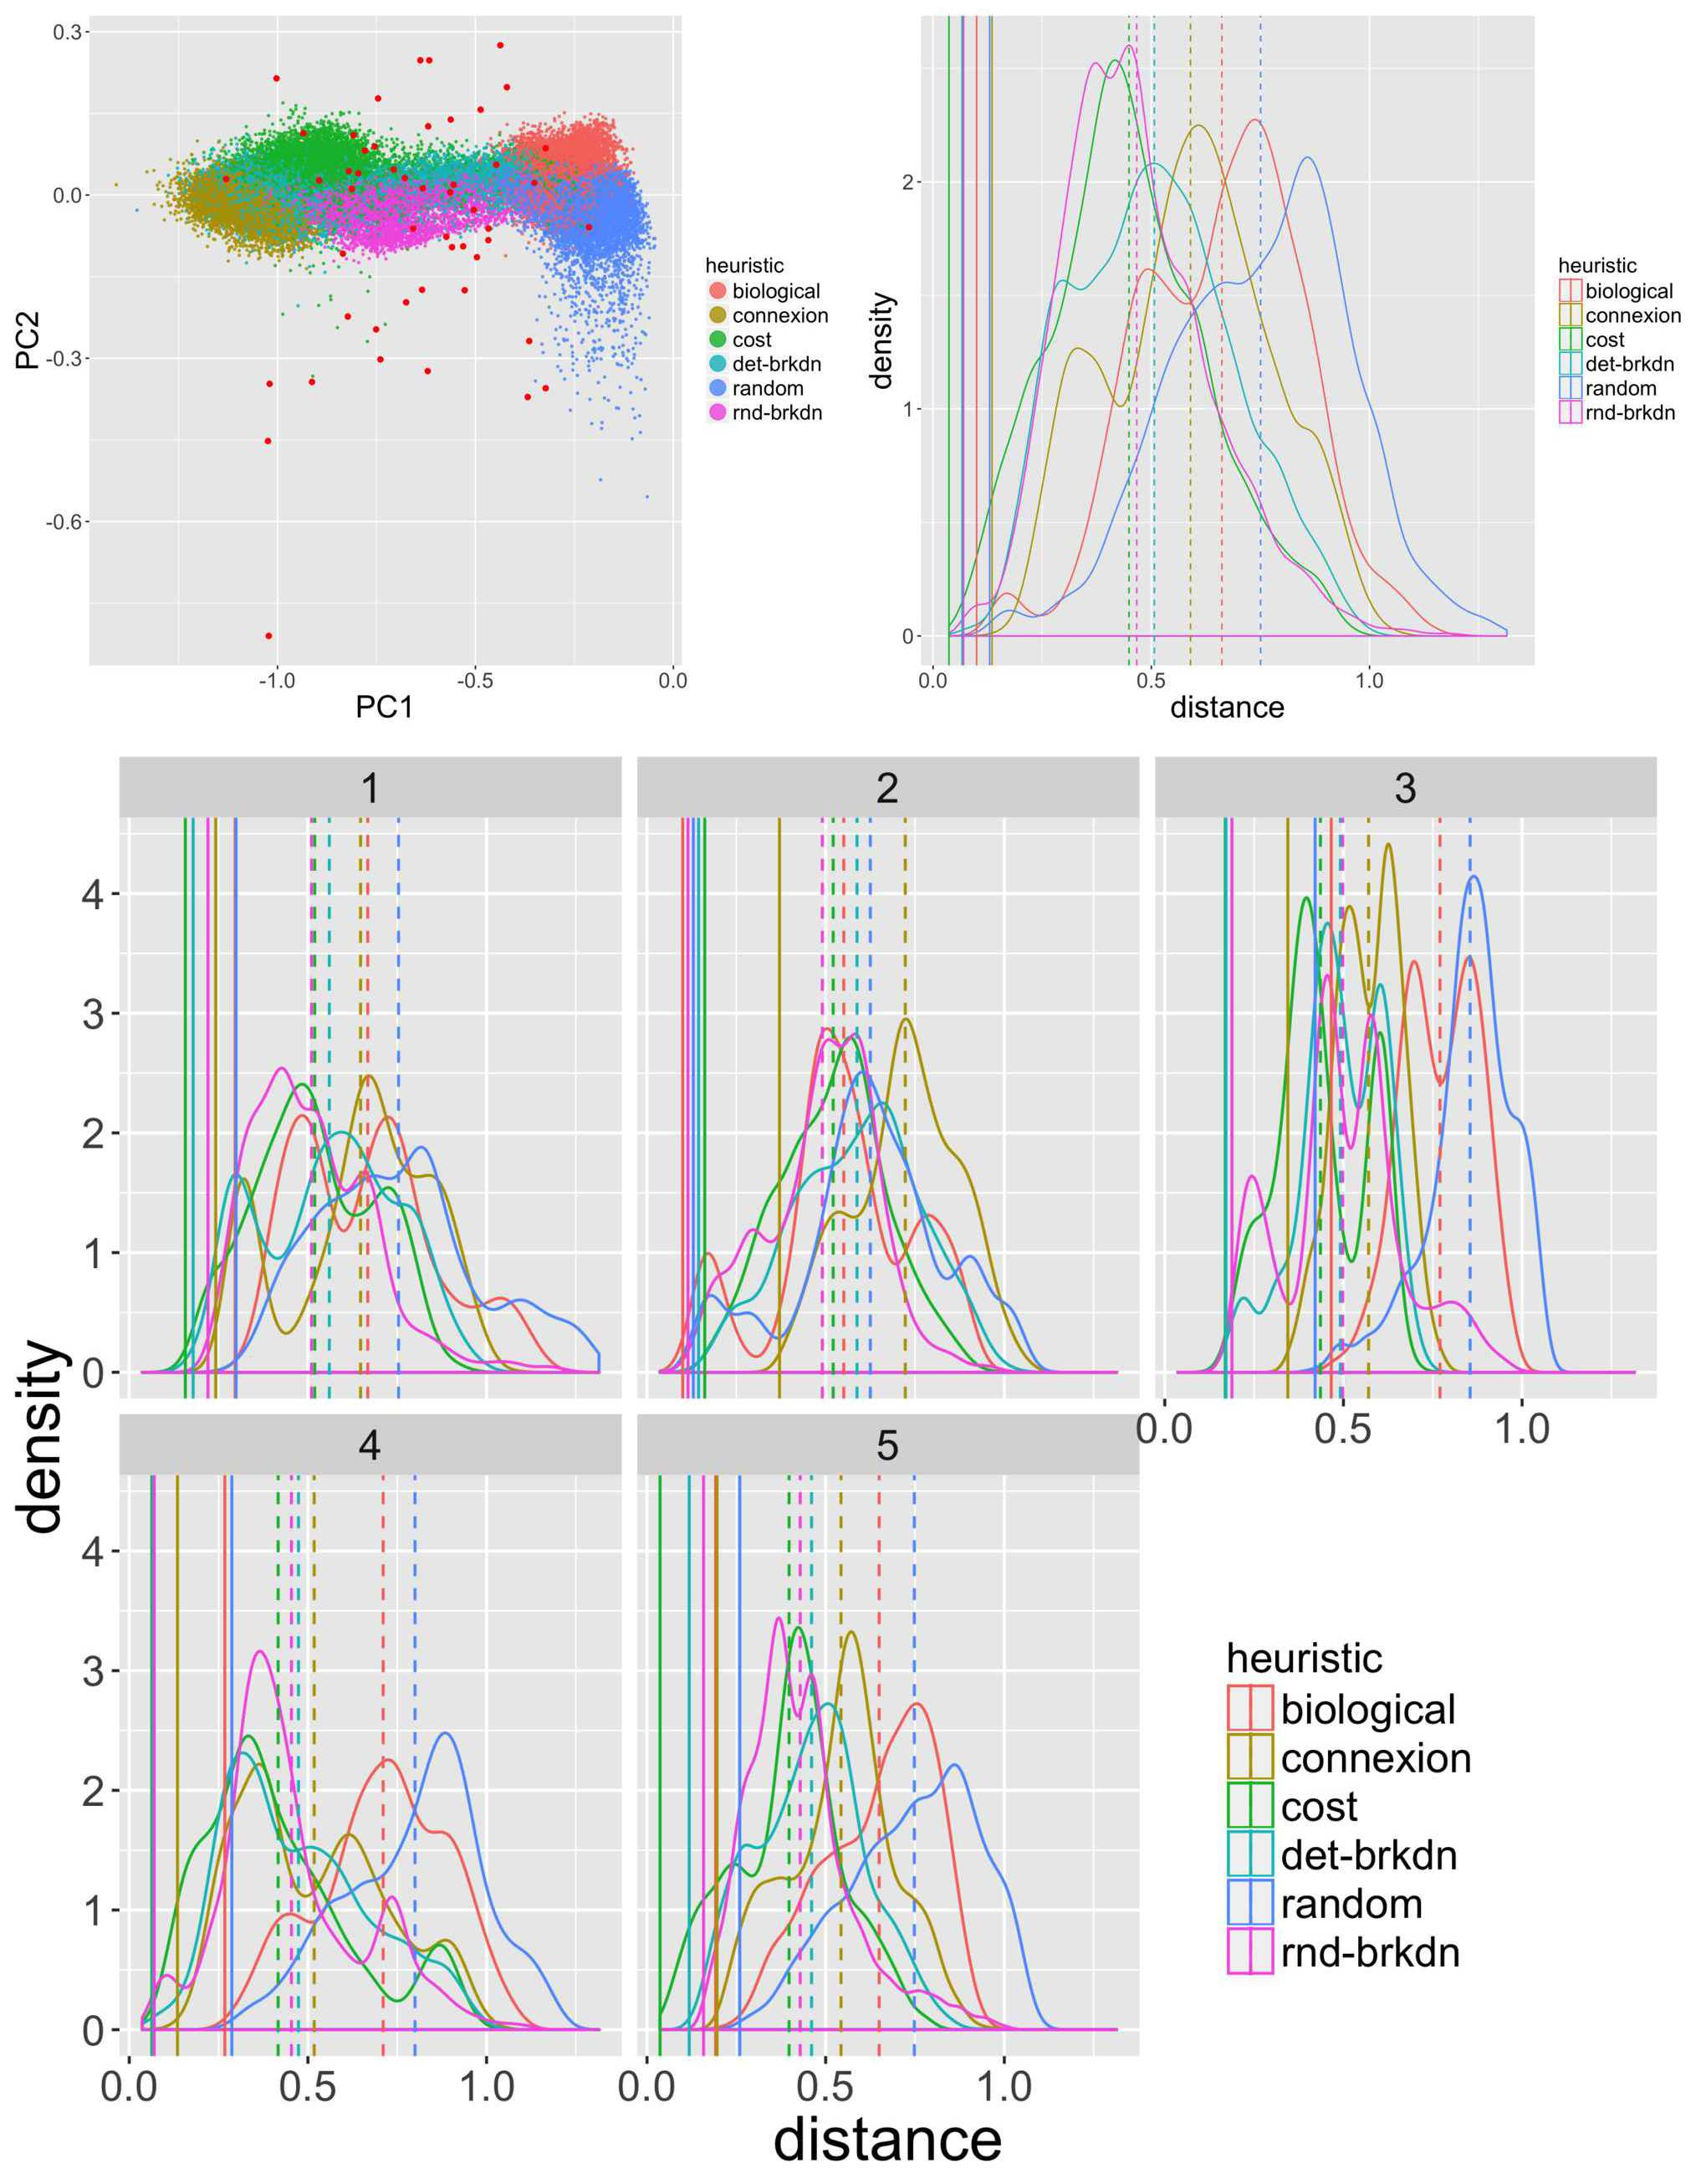
\includegraphics[width=\linewidth,height=0.85\textheight]{Figures/Final/7-1-2-fig-networkgrowth-realdistance}
\caption[Comparison to real networks][Comparaison aux réseaux réels]{\textbf{Comparison to real networks.} (\textit{Top Left}) Point clouds for simulated configurations (color in the legend) and for real configurations (in red), in a principal plan such that $PC1 = 0.12 \bar{bw} - 0.09 \bar{cl} + 0.98 \bar{l}$ and $PC2 = -0.20 \bar{bw} - 0.97 \bar{cl} - 0.06 \bar{l}$. (\textit{Top right}) Distribution of distances $d_{min}$ for all simulated points, for each heuristic (color). Dashed vertical lines give the average and solid lines the minimum for each distribution. (\textit{Bottom}) Same histograms, conditioned by morphological class for density distribution.\label{fig:networkgrowth:realdistance}}{\textbf{Comparaison aux réseaux réels.} (\textit{Haut Gauche}) Nuage de point des configurations simulées (couleur en légende) et des configurations réelles (en rouge), dans un plan principal tel que $PC1 = 0.12 \bar{bw} - 0.09 \bar{cl} + 0.98 \bar{l}$ et $PC2 = -0.20 \bar{bw} - 0.97 \bar{cl} - 0.06 \bar{l}$. (\textit{Haut Droite}) Distribution des distances $d_{min}$ pour l'ensemble des points simulés, par heuristique (couleur). Les lignes verticales pointillées donnent la moyenne et les lignes solides le minimum pour chaque distribution. (\textit{Bas}) Mêmes histogrammes, conditionnés par classe morphologique pour la distribution de densité.\label{fig:networkgrowth:realdistance}}
\end{figure}
%%%%%%%%%%%%%%%%%




\bpar{
We use the measures on real road networks obtained in~\ref{sec:staticcorrelations} to compute a distance of generated configurations to observed configurations, by considering real networks corresponding to density configurations used for initialization. We take for a given parameter point the minimum of the euclidian distance on vectors of indicators for all real points\footnote{What means that if $d(1,2) = \sqrt{(\bar{bw}_1 - \bar{bw}_2)^2 + (\bar{cl}_1 - \bar{cl}_2)^2 + (\bar{l}_1 - \bar{l}_2)^2}$, we consider $d_{min} = \min_j d(S,R_j)$ if $S$ is the simulated point and $R_j$ the set of real points. We keep here only the indicators $\bar{bw}$, $\bar{cl}$ and $\bar{l}$, for normalization reasons.}. This comparison is made possible since indicators are normalized, and indicators on real networks are comparable to indicators on synthetic networks.
}{
Nous utilisons les mesures sur réseaux routiers réels obtenues en~\ref{sec:staticcorrelations} pour calculer une distance des configurations générées aux configurations observées, en considérant les réseaux réels correspondant aux configurations de densité utilisées pour l'initialisation. Nous prenons pour un point de paramètre le minimum de distance euclidienne sur les vecteurs d'indicateurs pour l'ensemble des points réels\footnote{C'est-à-dire si $d(1,2) = \sqrt{(\bar{bw}_1 - \bar{bw}_2)^2 + (\bar{cl}_1 - \bar{cl}_2)^2 + (\bar{l}_1 - \bar{l}_2)^2}$, on considère $d_{min} = \min_j d(S,R_j)$ si $S$ est le point simulé et $R_j$ l'ensemble des points réels. Nous conservons ici uniquement les indicateurs $\bar{bw}$, $\bar{cl}$ et $\bar{l}$, pour des raisons de normalisation.}. Cette comparaison est possible car les indicateurs sont normalisés, et les indicateurs sur réseaux réels sont comparables aux indicateurs sur réseaux synthétiques.
}


%%%%%%%
% rq : should be only one point, the corresponding network ?
%%%%%%%


\bpar{
Comparison results to real points are given in Fig.~\ref{fig:networkgrowth:realdistance}. We give a representation as a point cloud and histograms for distributions of distances, on all grids and by morphological class. We observe that around ten real configuration (one fifth) fall far outside the point cloud. Once again, heuristics are complementary to approach a larger number of points. Concerning distances, the random heuristic is the worse in terms of mode and average, followed by the biological, the reference (connexion only), the deterministic breakdown and finally teh random-breakdown and the cost which are approximatively equivalent. All realize very low minimal distances.
}{
Les résultats de comparaison aux points réels sont donnés en Fig.~\ref{fig:networkgrowth:realdistance}. Nous donnons une représentation en nuage de points et les histogrammes de distribution des distances, sur l'ensemble des grilles et par classe morphologique. On constate qu'une dizaine de configurations réelles (1/5ème) se retrouvent à grande distance du nuage de points simulés, mais que les autres tombent à distance faible ou à l'intérieur du nuage de points. Encore une fois, les différentes heuristiques sont complémentaires pour approcher un plus grand nombre de points. Concernant les distances, l'aléatoire est le plus mauvais en termes de mode et de moyenne, suivi par le biologique, la référence (connection), la rupture déterministe puis la rupture aléatoire et le coût qui sont à peu près équivalentes. Elles réalisent toutes des distances minimales très faibles.
}


\bpar{
When conditioning by morphological classes, we see that classes 3, 4 and 5 give the most difficulties for all heuristics in terms of minima - they are indeed the configurations with very localized settlements or a diffuse population (see~\ref{app:sec:networkgrowth}): it is therefore easier to reproduce real network configurations in the case of polycentric structures. In all cases, the biological heuristic is not very efficient, but it is not directly possible to know if this is a consequence of its under-exploitation and its fixed parameters, or of its intrinsic dynamics.
}{
En conditionnant par les classes morphologiques, nous voyons que les classes 3, 4 et 5 donnent le plus de difficultés à l'ensemble des heuristiques en termes de minimum - or il s'agit des configurations avec établissements très localisés ou population diffuse (voir~\ref{app:sec:networkgrowth}) : il est donc plus facile de reproduire les configurations réelles de réseau dans le cas de structures polycentriques. Dans tous les cas, l'heuristique biologique est peu performante, mais il n'est pas directement possible de savoir si cela est dû à sa sous-exploration et aux paramètres fixés ou à sa dynamique intrinsèque.
}





% PCA full
%Rotation:
%                               PC1         PC2        PC3
%meanBwCentrality         0.1232342 -0.20841025 -0.9702466
%meanPathLength           0.9881203 -0.06469639  0.1394013
%meanClosenessCentrality -0.0918241 -0.97589935  0.1979616
%Importance of components:
%                          PC1     PC2     PC3
%Standard deviation     0.1676 0.02884 0.01203
%Proportion of Variance 0.9664 0.02860 0.00498
%Cumulative Proportion  0.9664 0.99502 1.00000
%


% Distances

%nres%>%group_by(heuristic)%>%summarise(distance=min(distance))
%1 biological 0.09990225
%2  connexion 0.13504050
%3       cost 0.03647362
%4  det-brkdn 0.06644744
%5     random 0.12968739
%6  rnd-brkdn 0.06994303
%
%nres%>%group_by(heuristic)%>%summarise(distance=mean(distance))
%
%1 biological 0.6616921
%2  connexion 0.5898689
%3       cost 0.4489075
%4  det-brkdn 0.5070177
%5     random 0.7504109
%6  rnd-brkdn 0.4666547
%
%nres%>%group_by(heuristic)%>%summarise(distance=median(distance))
%
%1 biological 0.6780299
%2  connexion 0.5973273
%3       cost 0.4359749
%4  det-brkdn 0.5024551
%5     random 0.7680822
%6  rnd-brkdn 0.4462033


%%%%%%%%%%%%%%%%%%%%%%%
\subsection{Discussion}{Discussion}


\bpar{
If the slime-mould model is able to generate robust networks in a simplified way, its use for planning has been questioned, in particular because it does not take into account external factors and the urban environment~\cite{adamatzky2010road}. Our results seem to confirm these analyses, since this heuristic is the least performing in terms of distance to real networks.
}{
Si le modèle slime-mould est capable de conduire de manière simplifiée à une génération de réseaux robustes, son utilisation pour la planification a été mise en question, notamment pour sa non prise en compte de facteurs extérieurs et de l'environnement urbain~\cite{adamatzky2010road}. Nos résultats semblent confirmer ces analyses, puisque cette heuristique est la moins performante au sens de la distance aux réseaux réels.
}


\bpar{
We have thus explored and compared different network generation heuristics, at a fixed density. We note the following points.
\begin{itemize}
	\item Different models produce networks that appear as complementary in an indicator space.
	\item Similarly, they are complementary to resemble configurations of real networks, while showing different performances. Very localized or diffuse density configurations correspond to networks that are more difficult to reproduce, in comparison to polycentric structures. 
\end{itemize}
}{
Nous avons donc exploré et comparé différentes heuristiques de génération de réseau, à densité fixée. Nous en retirons les enseignements suivants.
\begin{itemize}
	\item Les différents modèles produisent des réseaux qui apparaissent complémentaires dans un espace d'indicateurs.
	\item De même, ils sont complémentaires pour s'approcher des configurations des réseaux réels, tout en présentant des performances différentes. Des configurations de densité très localisées ou diffuses correspondent à des réseaux plus difficiles à reproduire, en comparaison aux structures polycentriques.
\end{itemize}
}

\stars


\bpar{
Armed with these network growth models, we will be able to couple them to a density model, in order to develop a co-evolution model at the mesoscopic scale, which will be the subject of the following section.
}{
Disposant de ces modèles de croissance de réseau, nous allons pouvoir les utiliser en couplage avec un modèle de densité, afin de développer un modèle de co-évolution à l'échelle mesoscopique, qui fera l'objet de la section suivante.
}


\stars



